\documentclass{scrartcl}

\usepackage{geometry}
\geometry{
	paper=a4paper, % Paper size
	top=2cm, % Top margin
	bottom=2cm, % Bottom margin
	left=2cm, % Left margin
	right=2cm, % Right margin
	headheight=0.75cm, % Header height
	footskip=1.5cm, % Space from the bottom margin to the baseline of the footer
	headsep=0.75cm, % Space from the top margin to the baseline of the header
	%showframe, % Uncomment to show how the type block is set on the page
}

\usepackage{tabularx}
\usepackage{booktabs}
\usepackage{blindtext}
% Character encoding
\usepackage[T1]{fontenc}
\usepackage[utf8]{inputenc}
% Mathematics packages from AMS
\usepackage{amsmath, amsfonts, amsthm, amssymb}
\usepackage{braket, nicefrac}
% International System of Units
\usepackage{siunitx}
% Lists / numbers
\usepackage{enumitem, multicol}
% Figure insertions
% Use option [H] to force the placement of a figure
\usepackage{graphicx, float}
\usepackage{keystroke}
\usepackage{pgfplots}\usepgfplotslibrary{units}\pgfplotsset{compat=1.16}
% Depth of the ToC
\setcounter{tocdepth}{3}
% Hyperlink References
\usepackage{hyperref}
\usepackage{enumitem}

\setlist{resume,leftmargin=8mm,itemsep=-0.5mm,topsep=-3mm}

% Storage Path for images
\graphicspath{{images/}}

\setkomafont{disposition}{\normalfont\bfseries}

% Environments
\renewenvironment{abstract}{
    \begin{center}
    {\Large \textbf{Abstract}}
    \vspace{0.5cm}
    \par\itshape
    \begin{minipage}{0.8\linewidth}}{\end{minipage}
    \noindent\ignorespaces
    \end{center}
}

\newenvironment{preface}{
  \begin{center}
    {\Large \textbf{Preface}}
    \vspace{0.5cm}
    \par
    \begin{minipage}{0.8\linewidth}}{\end{minipage}
    \noindent\ignorespaces
  \end{center}
}


\begin{document}
%Title of the report, name of coworkers and dates (of experiment and of report).
\begin{titlepage}
	\centering
	
\includegraphics[width=0.2\textwidth]{al-azhar.png}\par\vspace{12pt}
	{\LARGE Al-Azhar University \par}\vspace{3pt}
	{\Large Faculty of Engineering \par}
	{\Large Computers \& Systems Engineering Department \par}\vspace{12pt}
	\vfill
	{\huge\bfseries\scshape Web Page Ranking \par}\vspace{8pt}
  {\scshape SEO Suggestion Search Engine Project \par}\vspace{8pt}
  {\itshape (System Design Report) \par}
	\vfill
	{\Large\texttt{Contributors:} \\[12pt]
    \Large\itshape\ttfamily
    \begin{tabular}{ll}
      55 & Abd El-Twab M. Fakhry \\
      56 & Abd El-Hameed Hassan \\
      57 & Abd El-Khalek Alashker \\
      58 & Abdulrhman Ahmed Khalifa \\
      59 & Abdurrahman Gamal \\
      60 & Abdurrahman Ramadan Zaki \\
    \end{tabular}
  }\par
	\vspace{1cm}
	\vfill
  {\Large\texttt{Supervised by:} \\
	\texttt{Dr. Muhammad Atef} \par}
  \vfill
  {\large \today \par}
\end{titlepage}

\newpage

\tableofcontents

\newpage

\section{Introduction}

Our Page Ranking Project has the basic search functionality for searching website data. Furthermore, The Page Rank Project keeps track of visited website URLs and updates that number in the database automatically when the user clicks on that website URL. Additionally, website owners can find suitable keywords and meta-description for their website. The system also has the page rank calculations feature, which is only visible to the admin.

\section{User Stories}

The system has two main actors: The administrator and the User.
In the following set of tables, we describe in detail the user story.
Each user story is attached to it a UI design for better understanding. Furthermore, the user story acceptance criteria.

\begin{table}[H]
  \caption{Administrator login, user story 1}
  \begin{tabular}{p{0.20\linewidth} | p{0.74\linewidth}}
    \toprule
    ID & US\_1
    \\\midrule
    Summary & \textbf{Administrator login}
    \\\hline
    Description & \textbf{As an} administrator, \textbf{I want} to login into the system, \textbf{So that} I can enter the admin area.
    \\\hline
    Priority & \textcolor{red}{Highest}
    \\\hline
    Story Points & 3
    \\\hline
    UI/UX Attachment & {
                       \begin{center}
                         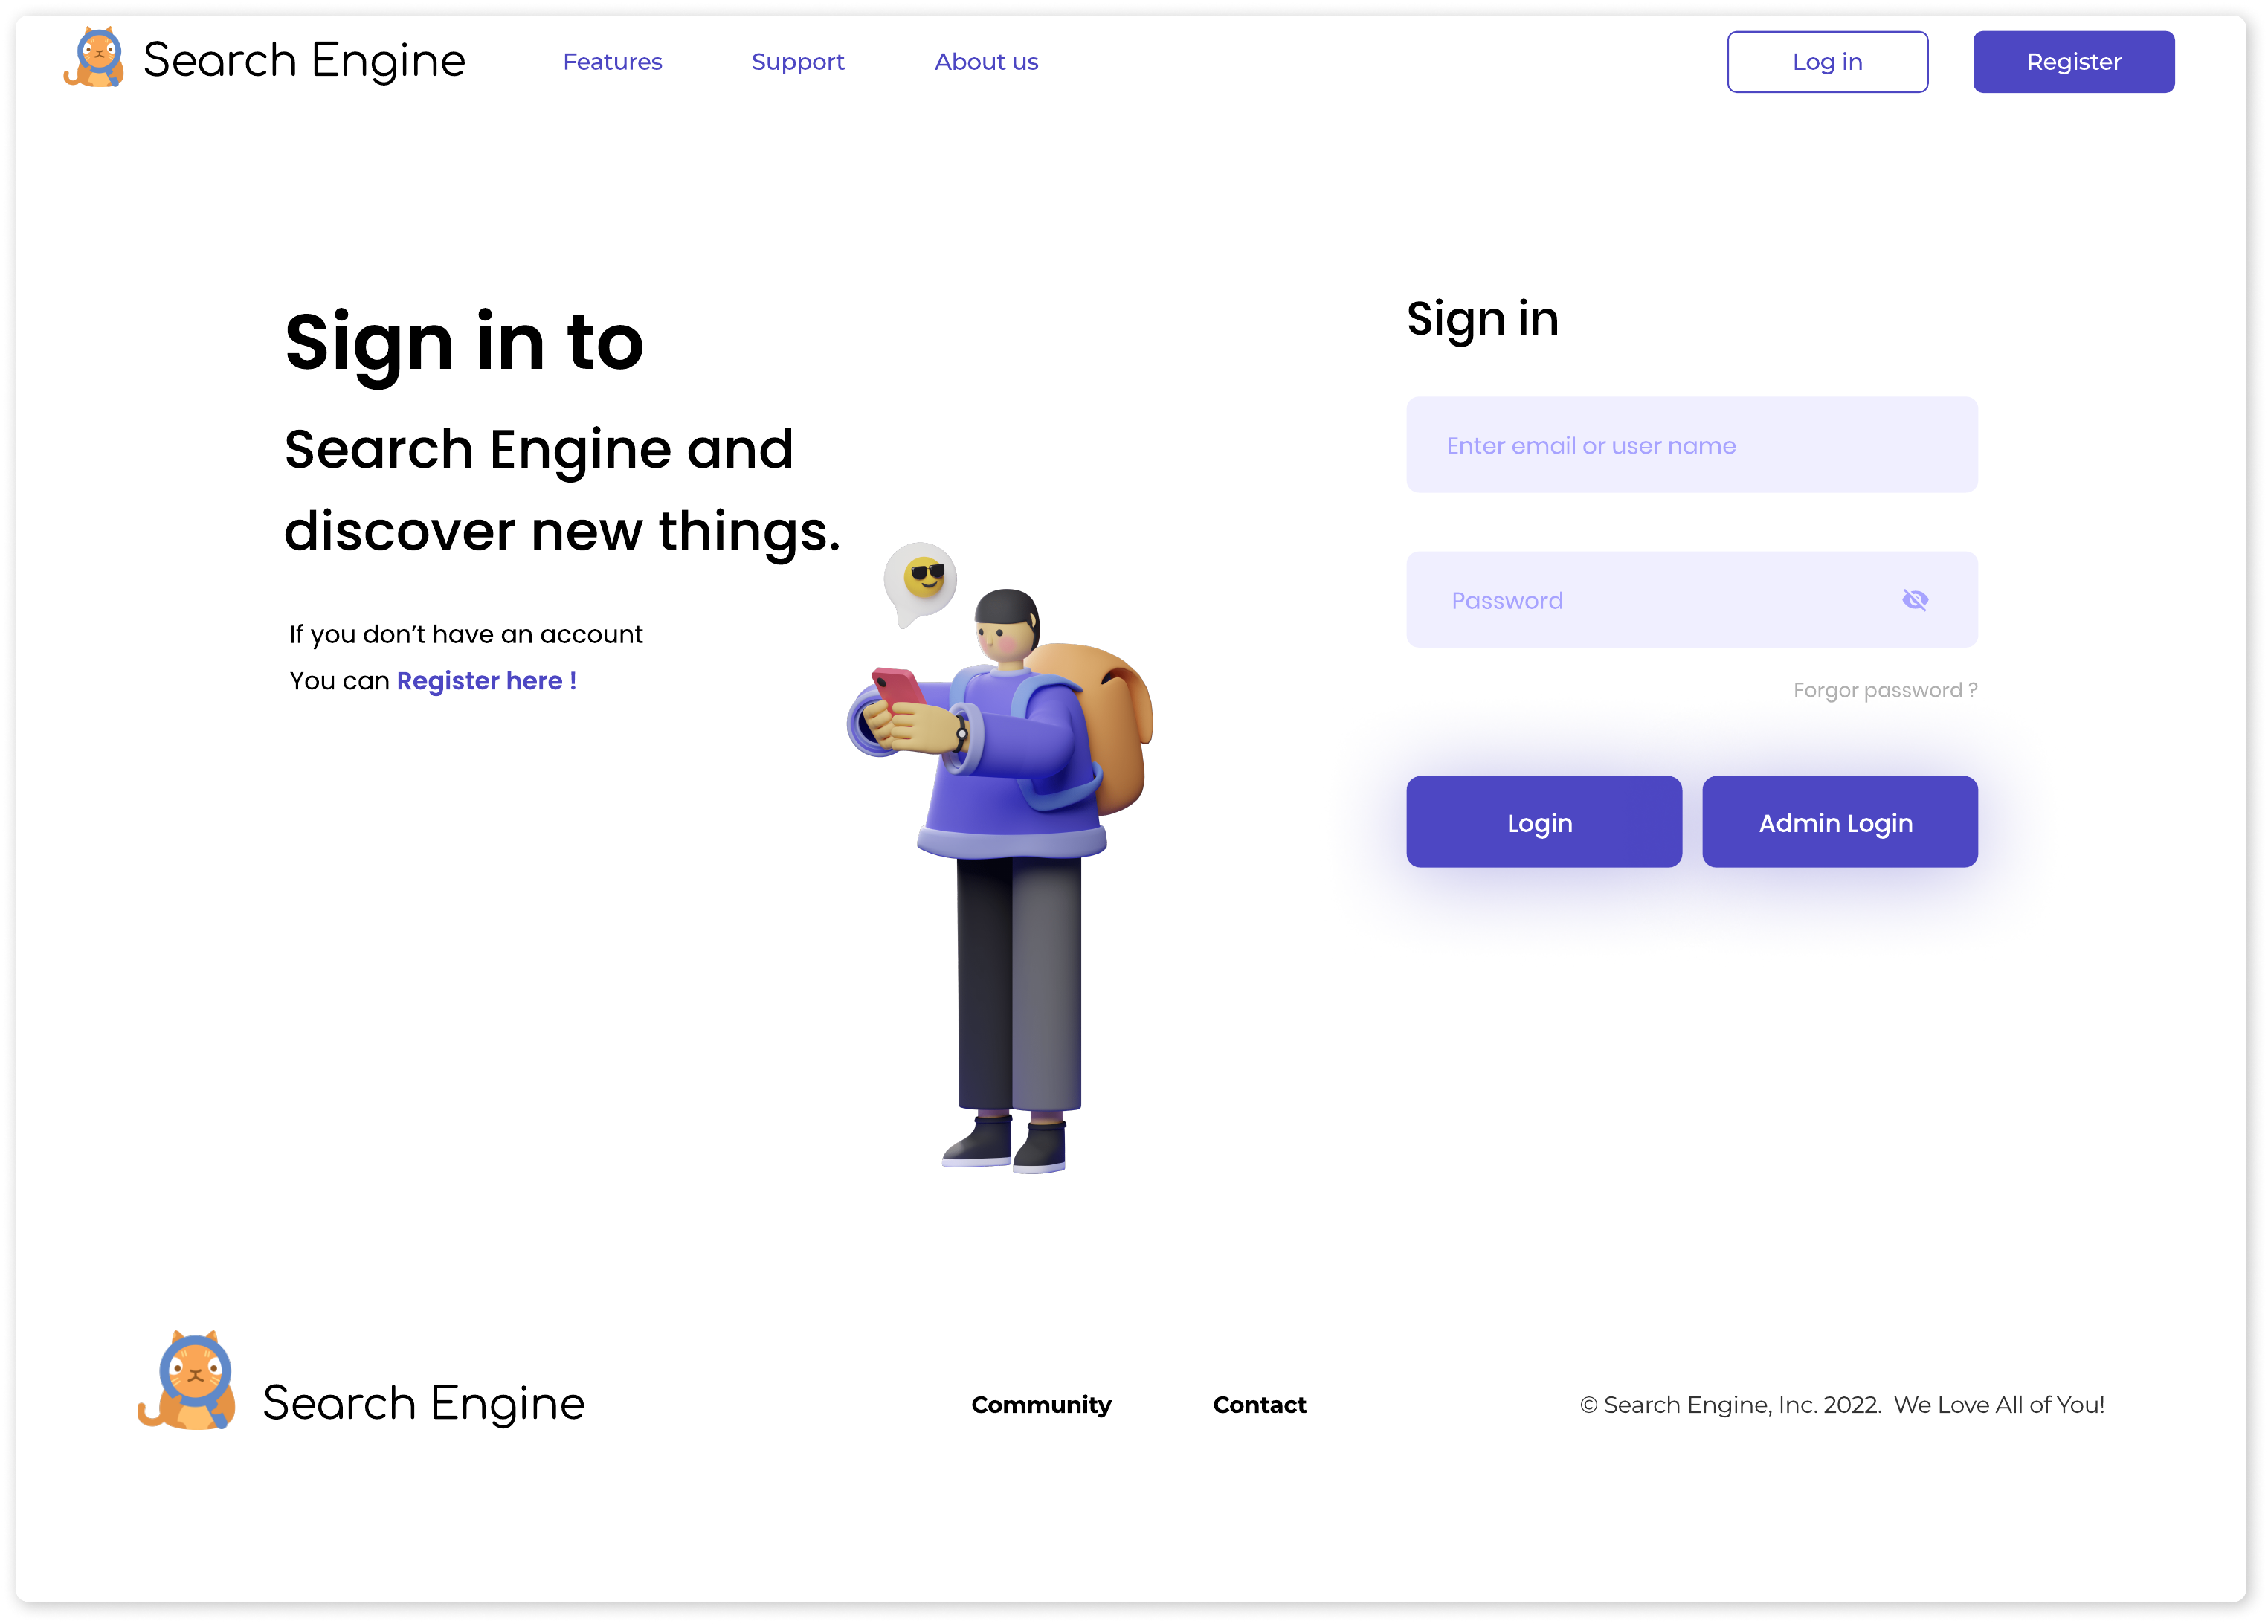
\includegraphics[scale=0.23]{login.pdf}
                       \end{center}
                       }
    \\\hline
    Pre Conditions & {
                     \begin{itemize}
                     \item The administrator should have the authorization credentials to enter the admin area.
                     \end{itemize}
                     }\vspace*{-\baselineskip}
    \\\hline
    Acceptance Criteria & {
                          \begin{center}
                            \textbf{Senario: } Admin successfully login into the system. \\
                          \end{center}
    \textbf{Given} The admin navigates to the login page, \textbf{When} The admin enters a valid username and password \textbf{And} The admin clicks on the Admin Login button, \textbf{Then} The admin will successfully login into the system.
    }
    \\\bottomrule
  \end{tabular}
\end{table}

\begin{table}[H]
  \caption{Feeding a new website URL to search, user story 2}
  \begin{tabular}{p{0.20\linewidth} | p{0.74\linewidth}}
    \toprule
    ID & US\_2
    \\\midrule
    Summary & \textbf{Feeds website URls}
    \\\hline
    Description & \textbf{As an} administrator, \textbf{I want} to be able to feed the database website URLs and their metadata, \textbf{So that} the system can use them to search the user query.
    \\\hline
    Priority & \textcolor{red}{Highest}
    \\\hline
    Story Points & 5
    \\\hline
    UI/UX Attachment & {
                       \begin{center}
                         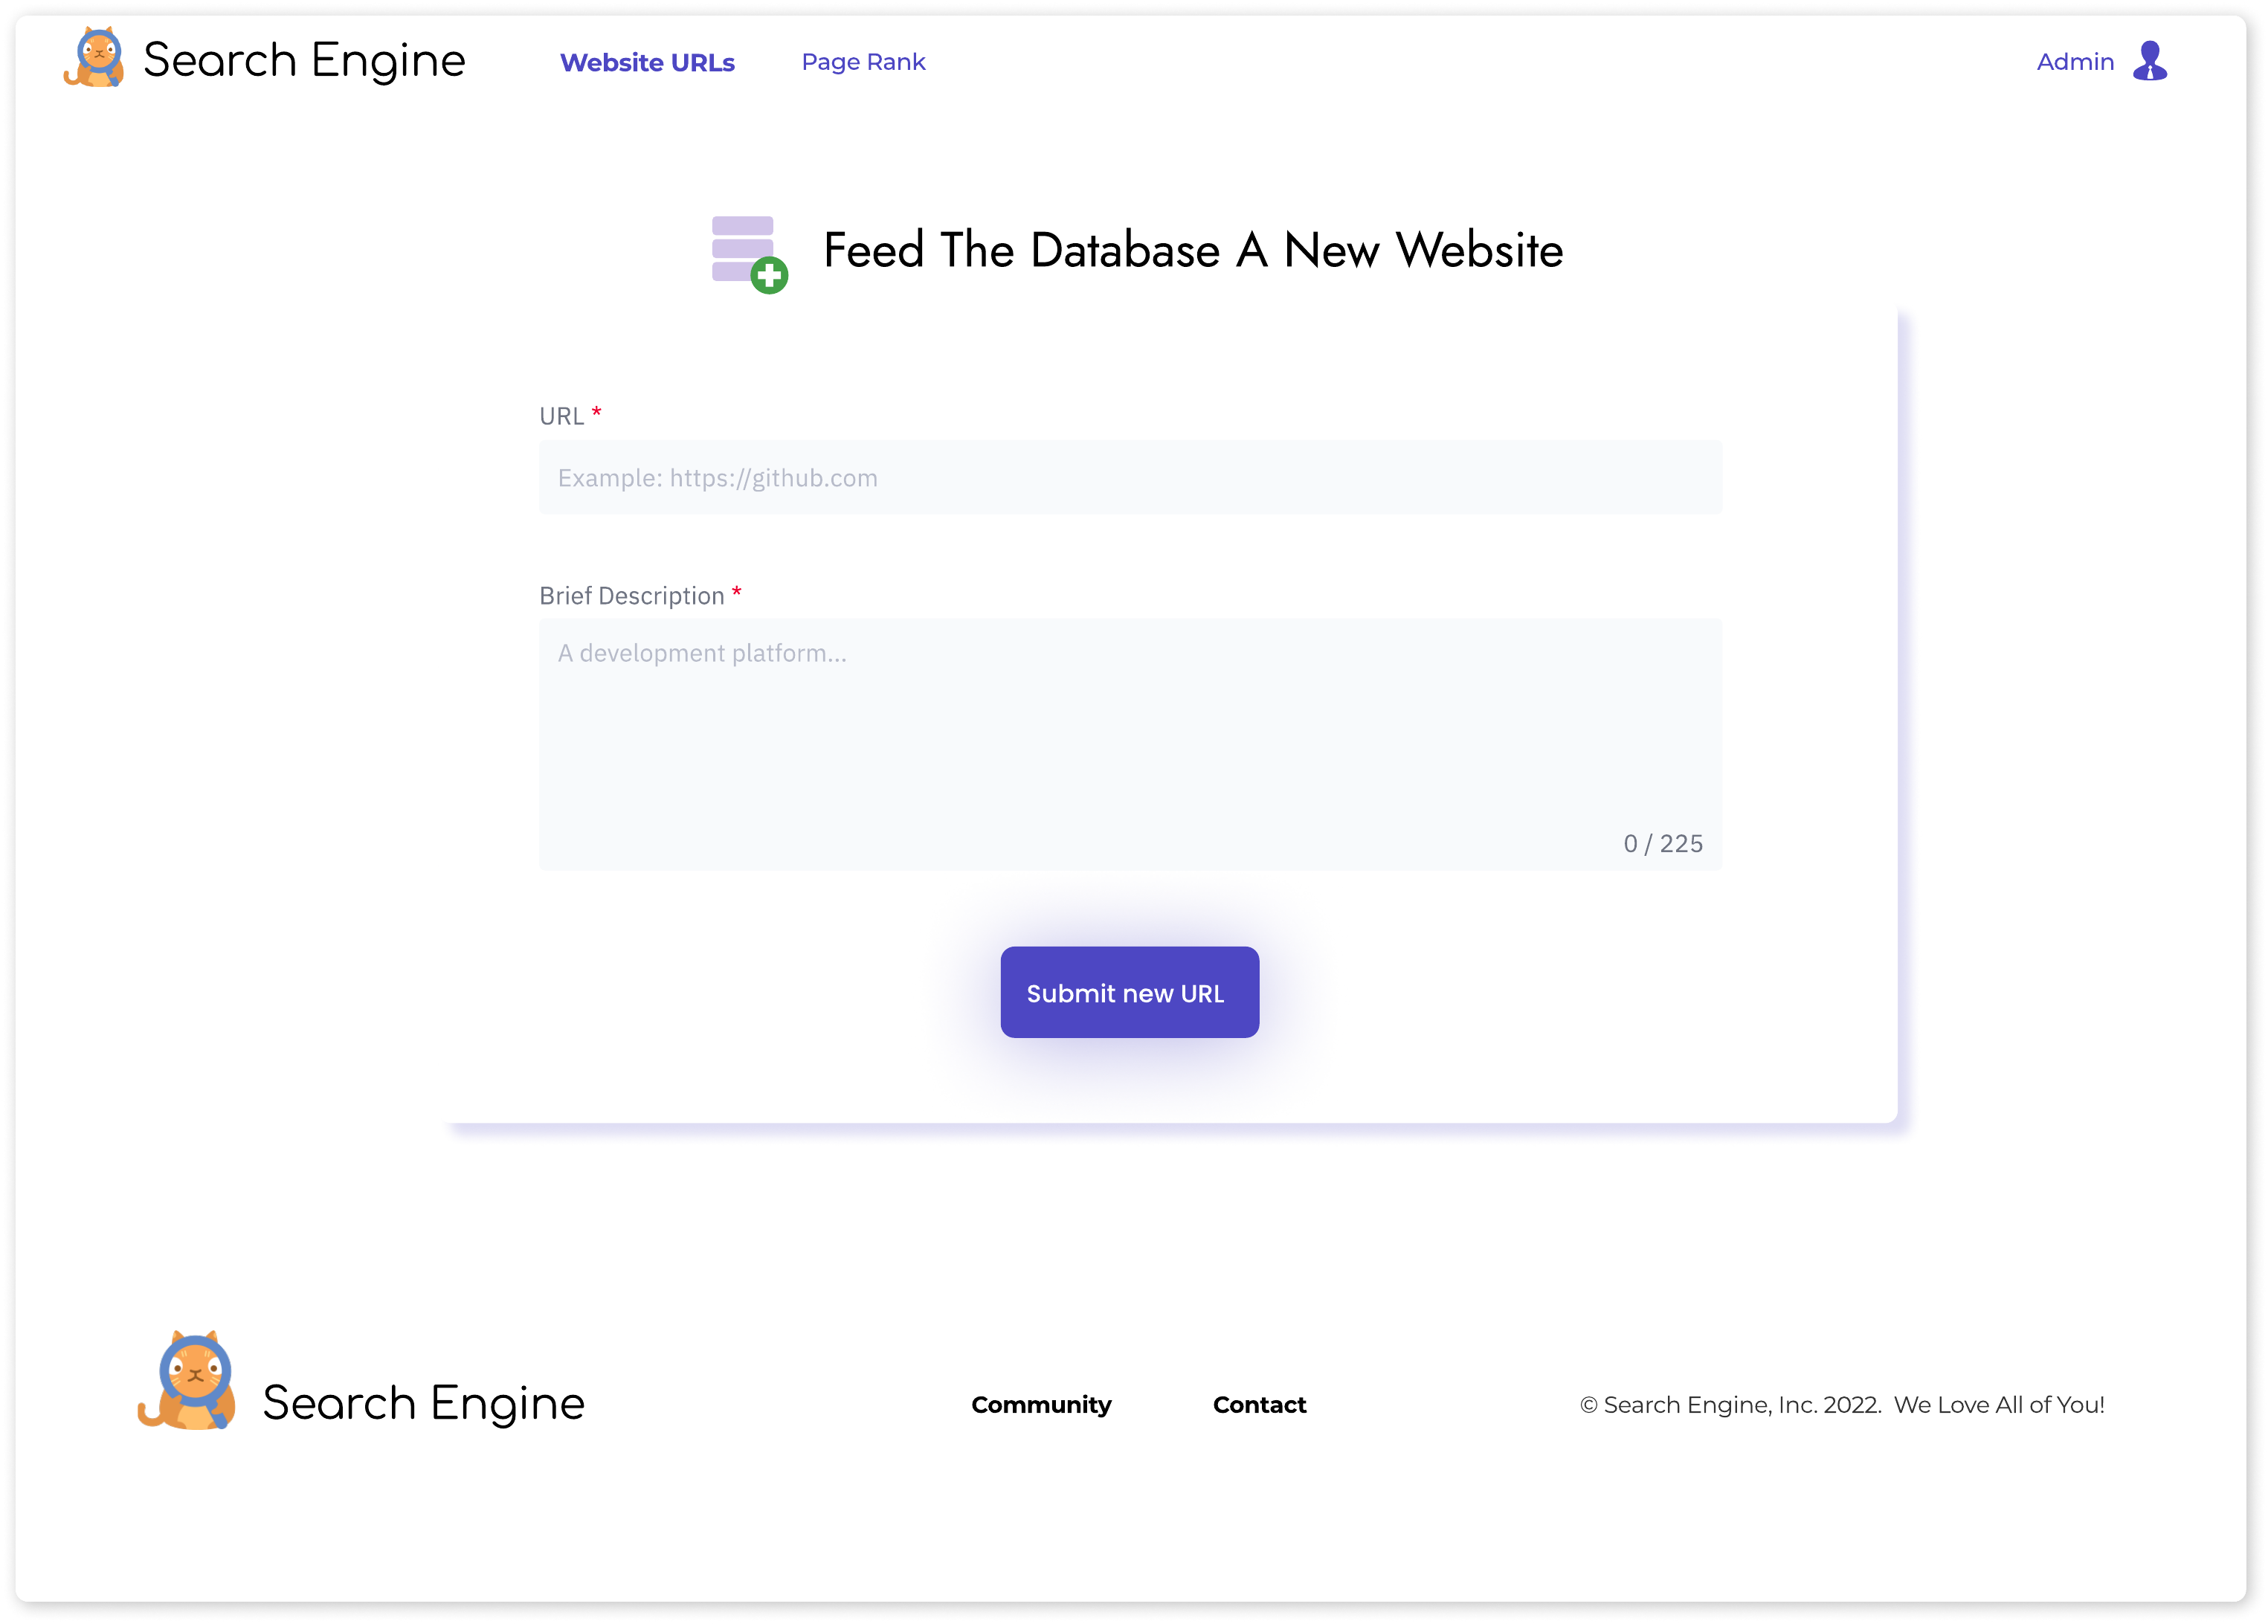
\includegraphics[scale=0.23]{website-urls.pdf}
                       \end{center}
                       }
    \\\hline
    Pre Conditions & {
                     \begin{itemize}
                     \item US\_1
                     \end{itemize}
                     }\vspace*{-\baselineskip}
    \\\hline
    Acceptance Criteria & {
                          \begin{center}
                            \textbf{Senario: } Admin successfully feeds a website URL and its metadata. \\
                          \end{center}
    \textbf{Given} The admin navigates to the website URLs page, \textbf{When} The admin enters a valid URL and metadata \textbf{And} The admin clicks on submit new URL button, \textbf{Then} The system will add new website to the database.
    }
    \\\bottomrule
  \end{tabular}
\end{table}

\begin{table}[H]
  \caption{Page rank calculations, user story 3}
  \begin{tabular}{p{0.20\linewidth} | p{0.74\linewidth}}
    \toprule
    ID & US\_3
    \\\midrule
    Summary & \textbf{Page rank calculations}
    \\\hline
    Description & \textbf{As an} administrator, \textbf{I want} to view the page rank calculations, \textbf{So that} I can optimize the search functionality.
    \\\hline
    Priority & \textcolor{orange}{High}
    \\\hline
    Story Points & 8
    \\\hline
    UI/UX Attachment & {
                       \begin{center}
                         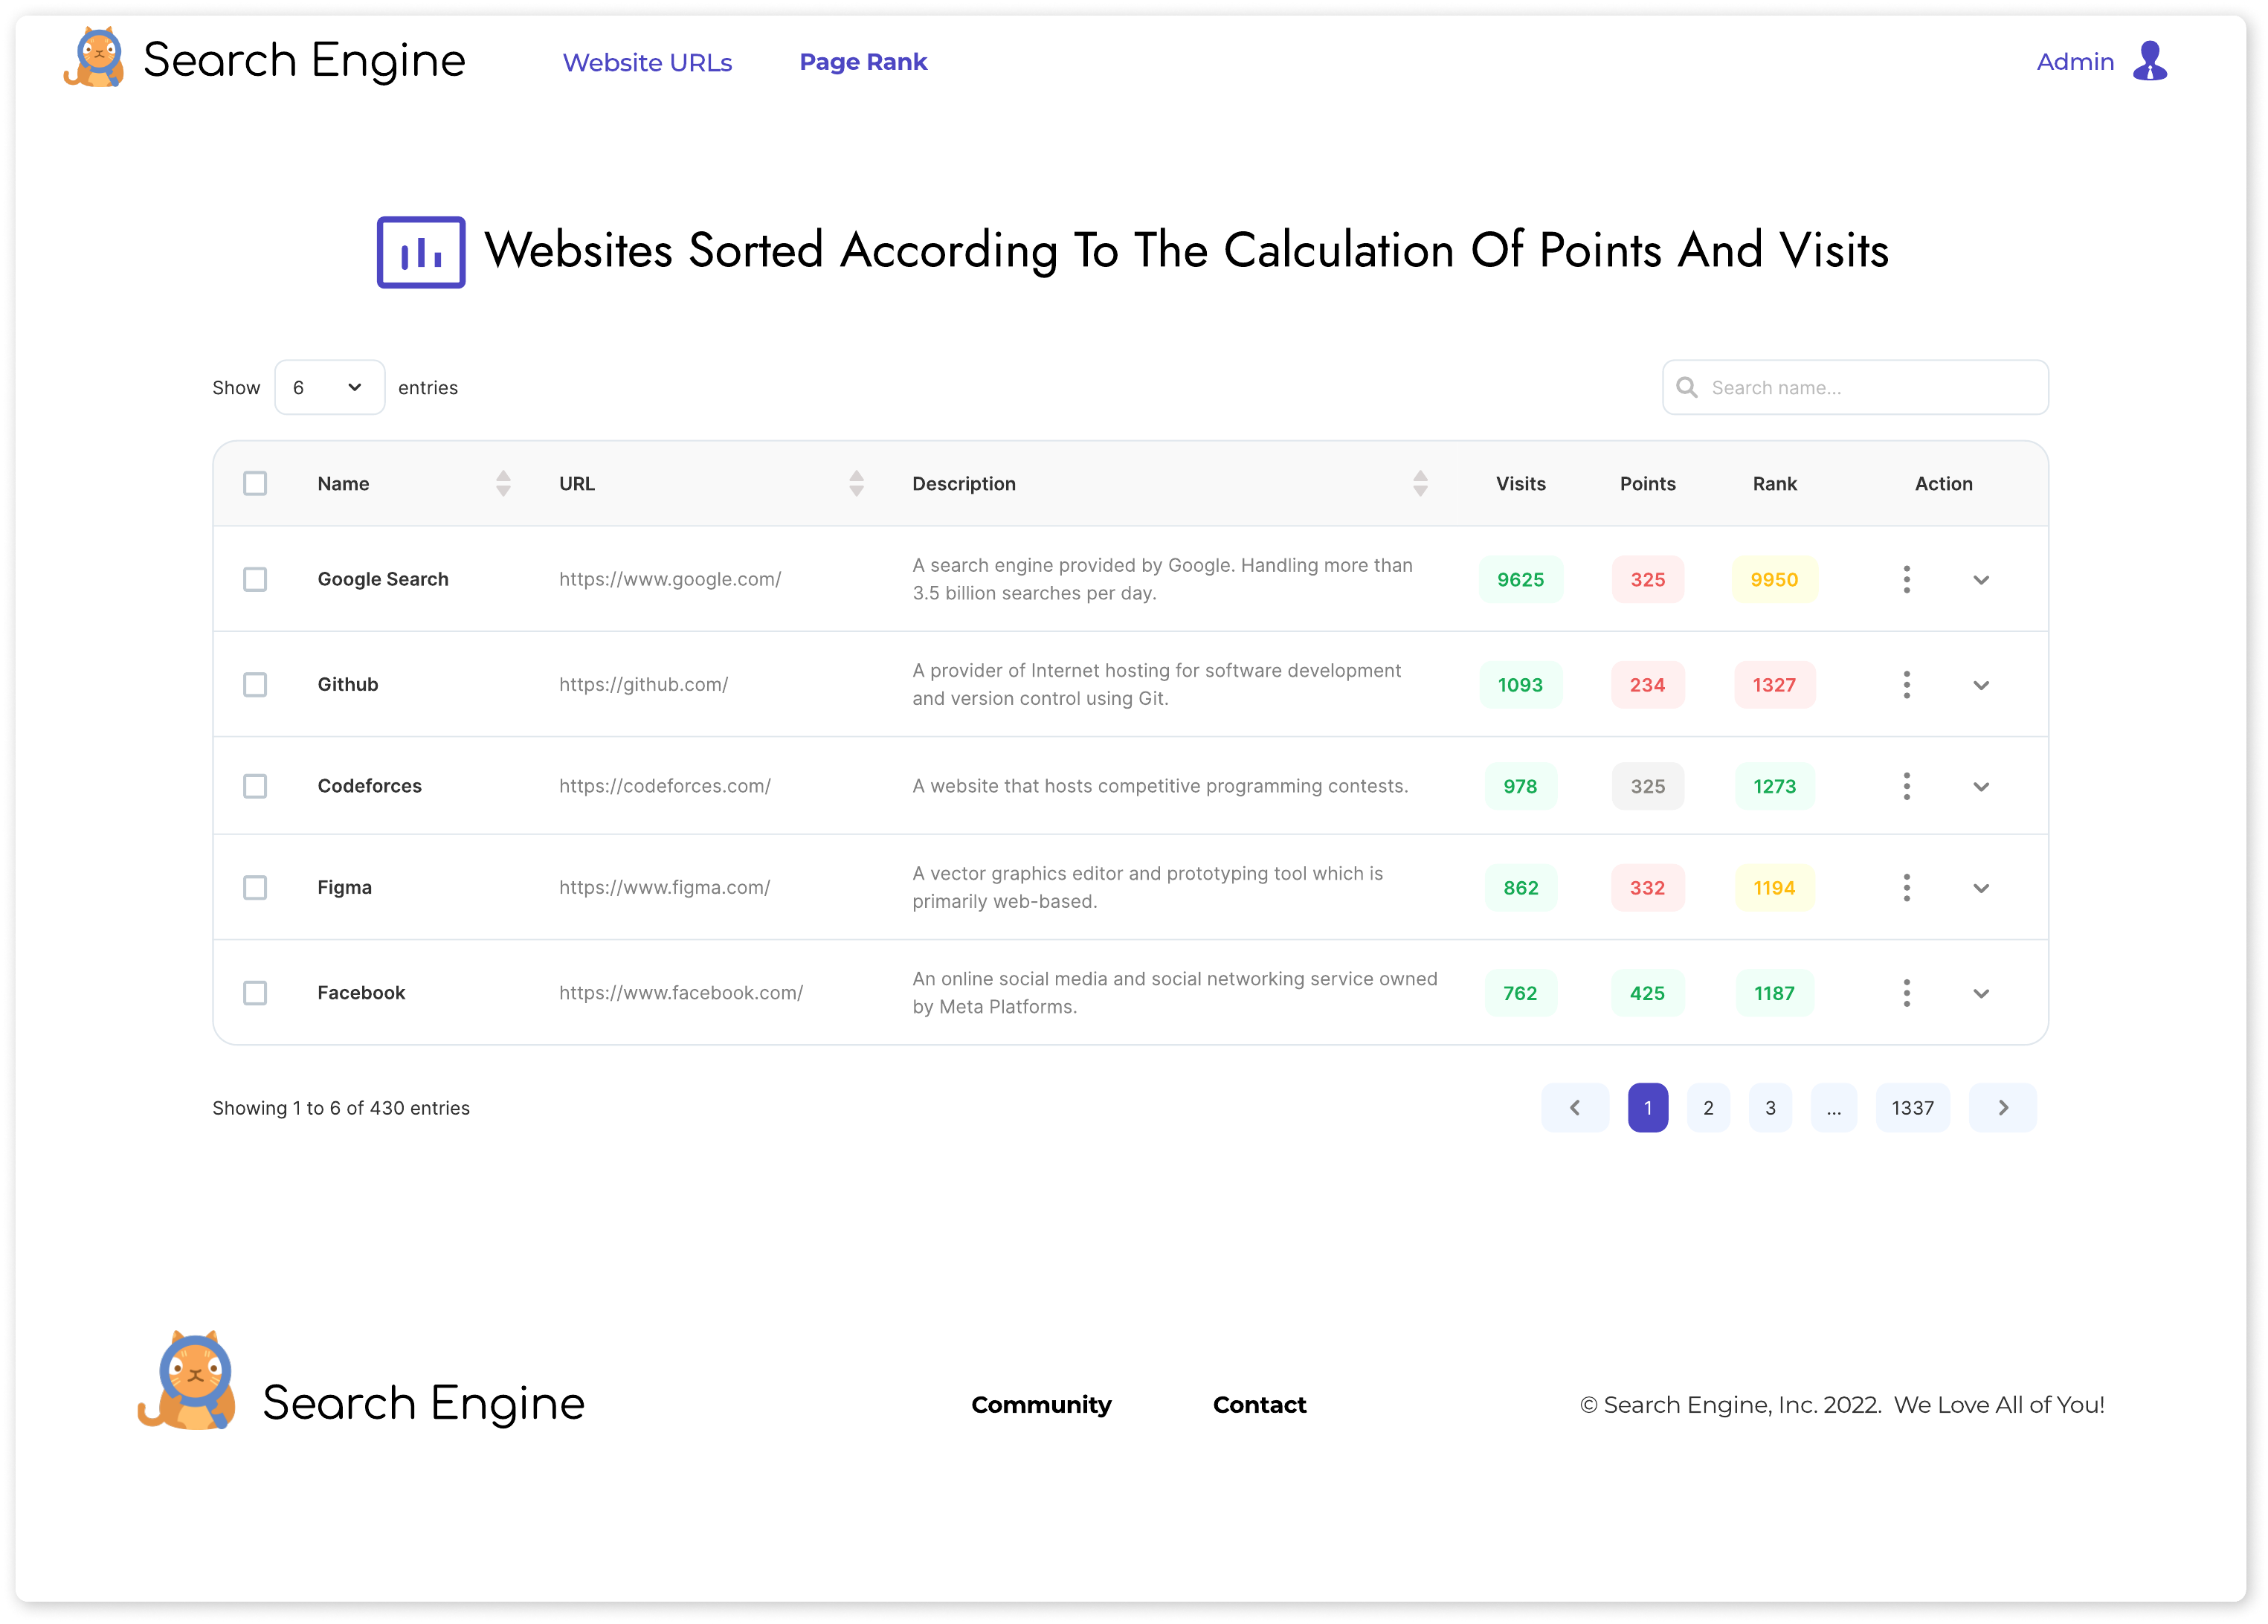
\includegraphics[scale=0.23]{page-rank.pdf}
                       \end{center}
                       }
    \\\hline
    Pre Conditions & {
                     \begin{itemize}
                     \item US\_1
                     \end{itemize}
                     }\vspace*{-\baselineskip}
    \\\hline
    Acceptance Criteria & {
                          \begin{center}
                            \textbf{Senario: } Admin will be able to display the page rank list. \\
                          \end{center}
    \textbf{Given} The admin navigates to the Page Rank page, \textbf{Then} The system will list out all pages sorted in descending order according to their points and visits.
    }
    \\\bottomrule
  \end{tabular}
\end{table}

\begin{table}[H]
  \caption{User registration, user story 4}
  \begin{tabular}{p{0.20\linewidth} | p{0.74\linewidth}}
    \toprule
    ID & US\_4
    \\\midrule
    Summary & \textbf{User registration}
    \\\hline
    Description & \textbf{As a} user, \textbf{I want} to be able to register to the system, \textbf{So that} I can use system functionality.
    \\\hline
    Priority & \textcolor{red}{Highest}
    \\\hline
    Story Points & 3
    \\\hline
    UI/UX Attachment & {
                       \begin{center}
                         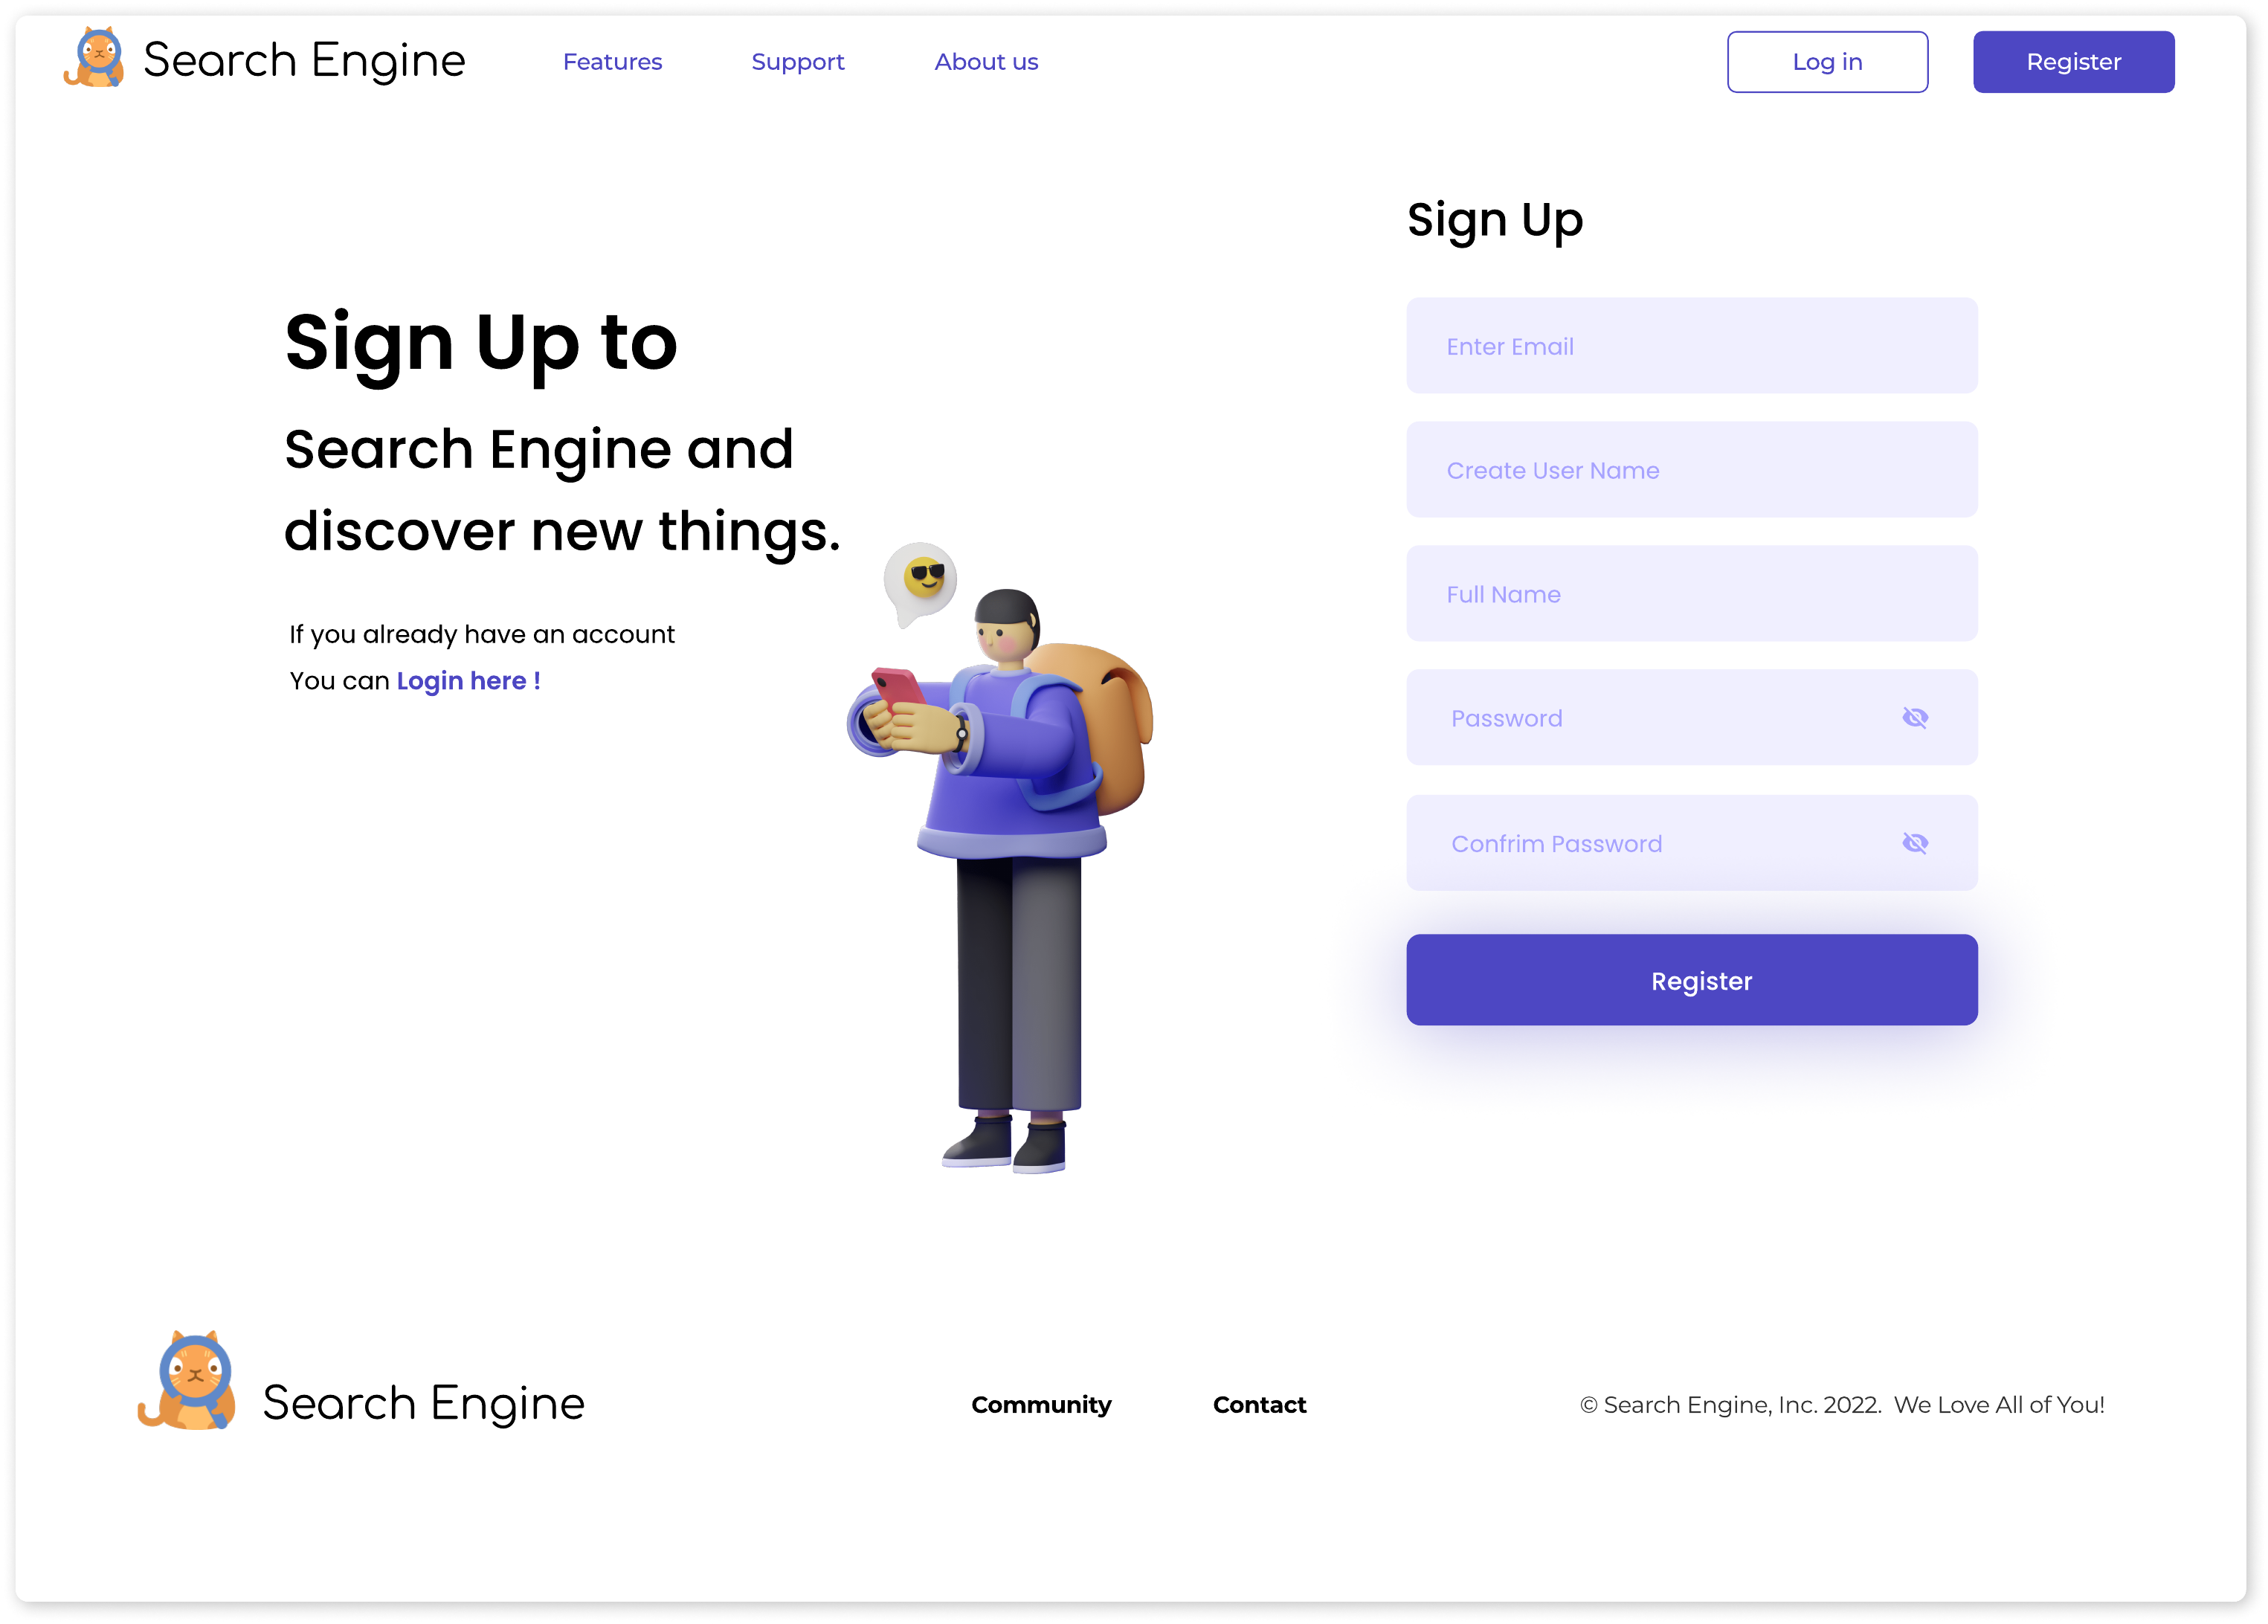
\includegraphics[scale=0.23]{register.pdf}
                       \end{center}
                       }
    \\\hline
    Pre Conditions & -
    \\\hline
    Acceptance Criteria & {
                          \begin{center}
                            \textbf{Senario: } User successfully register to the system. \\
                          \end{center}
    \textbf{Given} The user navigates to the sign-up page, \textbf{When} The user enters a valid email, username, full name, password, and confirm password correctly \textbf{And} The user clicks on the Register button, \textbf{Then} The system will successfully register the user into the system.
    }
    \\\bottomrule
  \end{tabular}
\end{table}

\begin{table}[H]
  \caption{User login, user story 5}
  \begin{tabular}{p{0.20\linewidth} | p{0.74\linewidth}}
    \toprule
    ID & US\_5
    \\\midrule
    Summary & \textbf{User login}
    \\\hline
    Description & \textbf{As a} user, \textbf{I want} to login into the system, \textbf{So that} I can search for specific topics and finding suitable keywords for my website.
    \\\hline
    Priority & \textcolor{red}{Highest}
    \\\hline
    Story Points & 2
    \\\hline
    UI/UX Attachment & {
                       \begin{center}
                         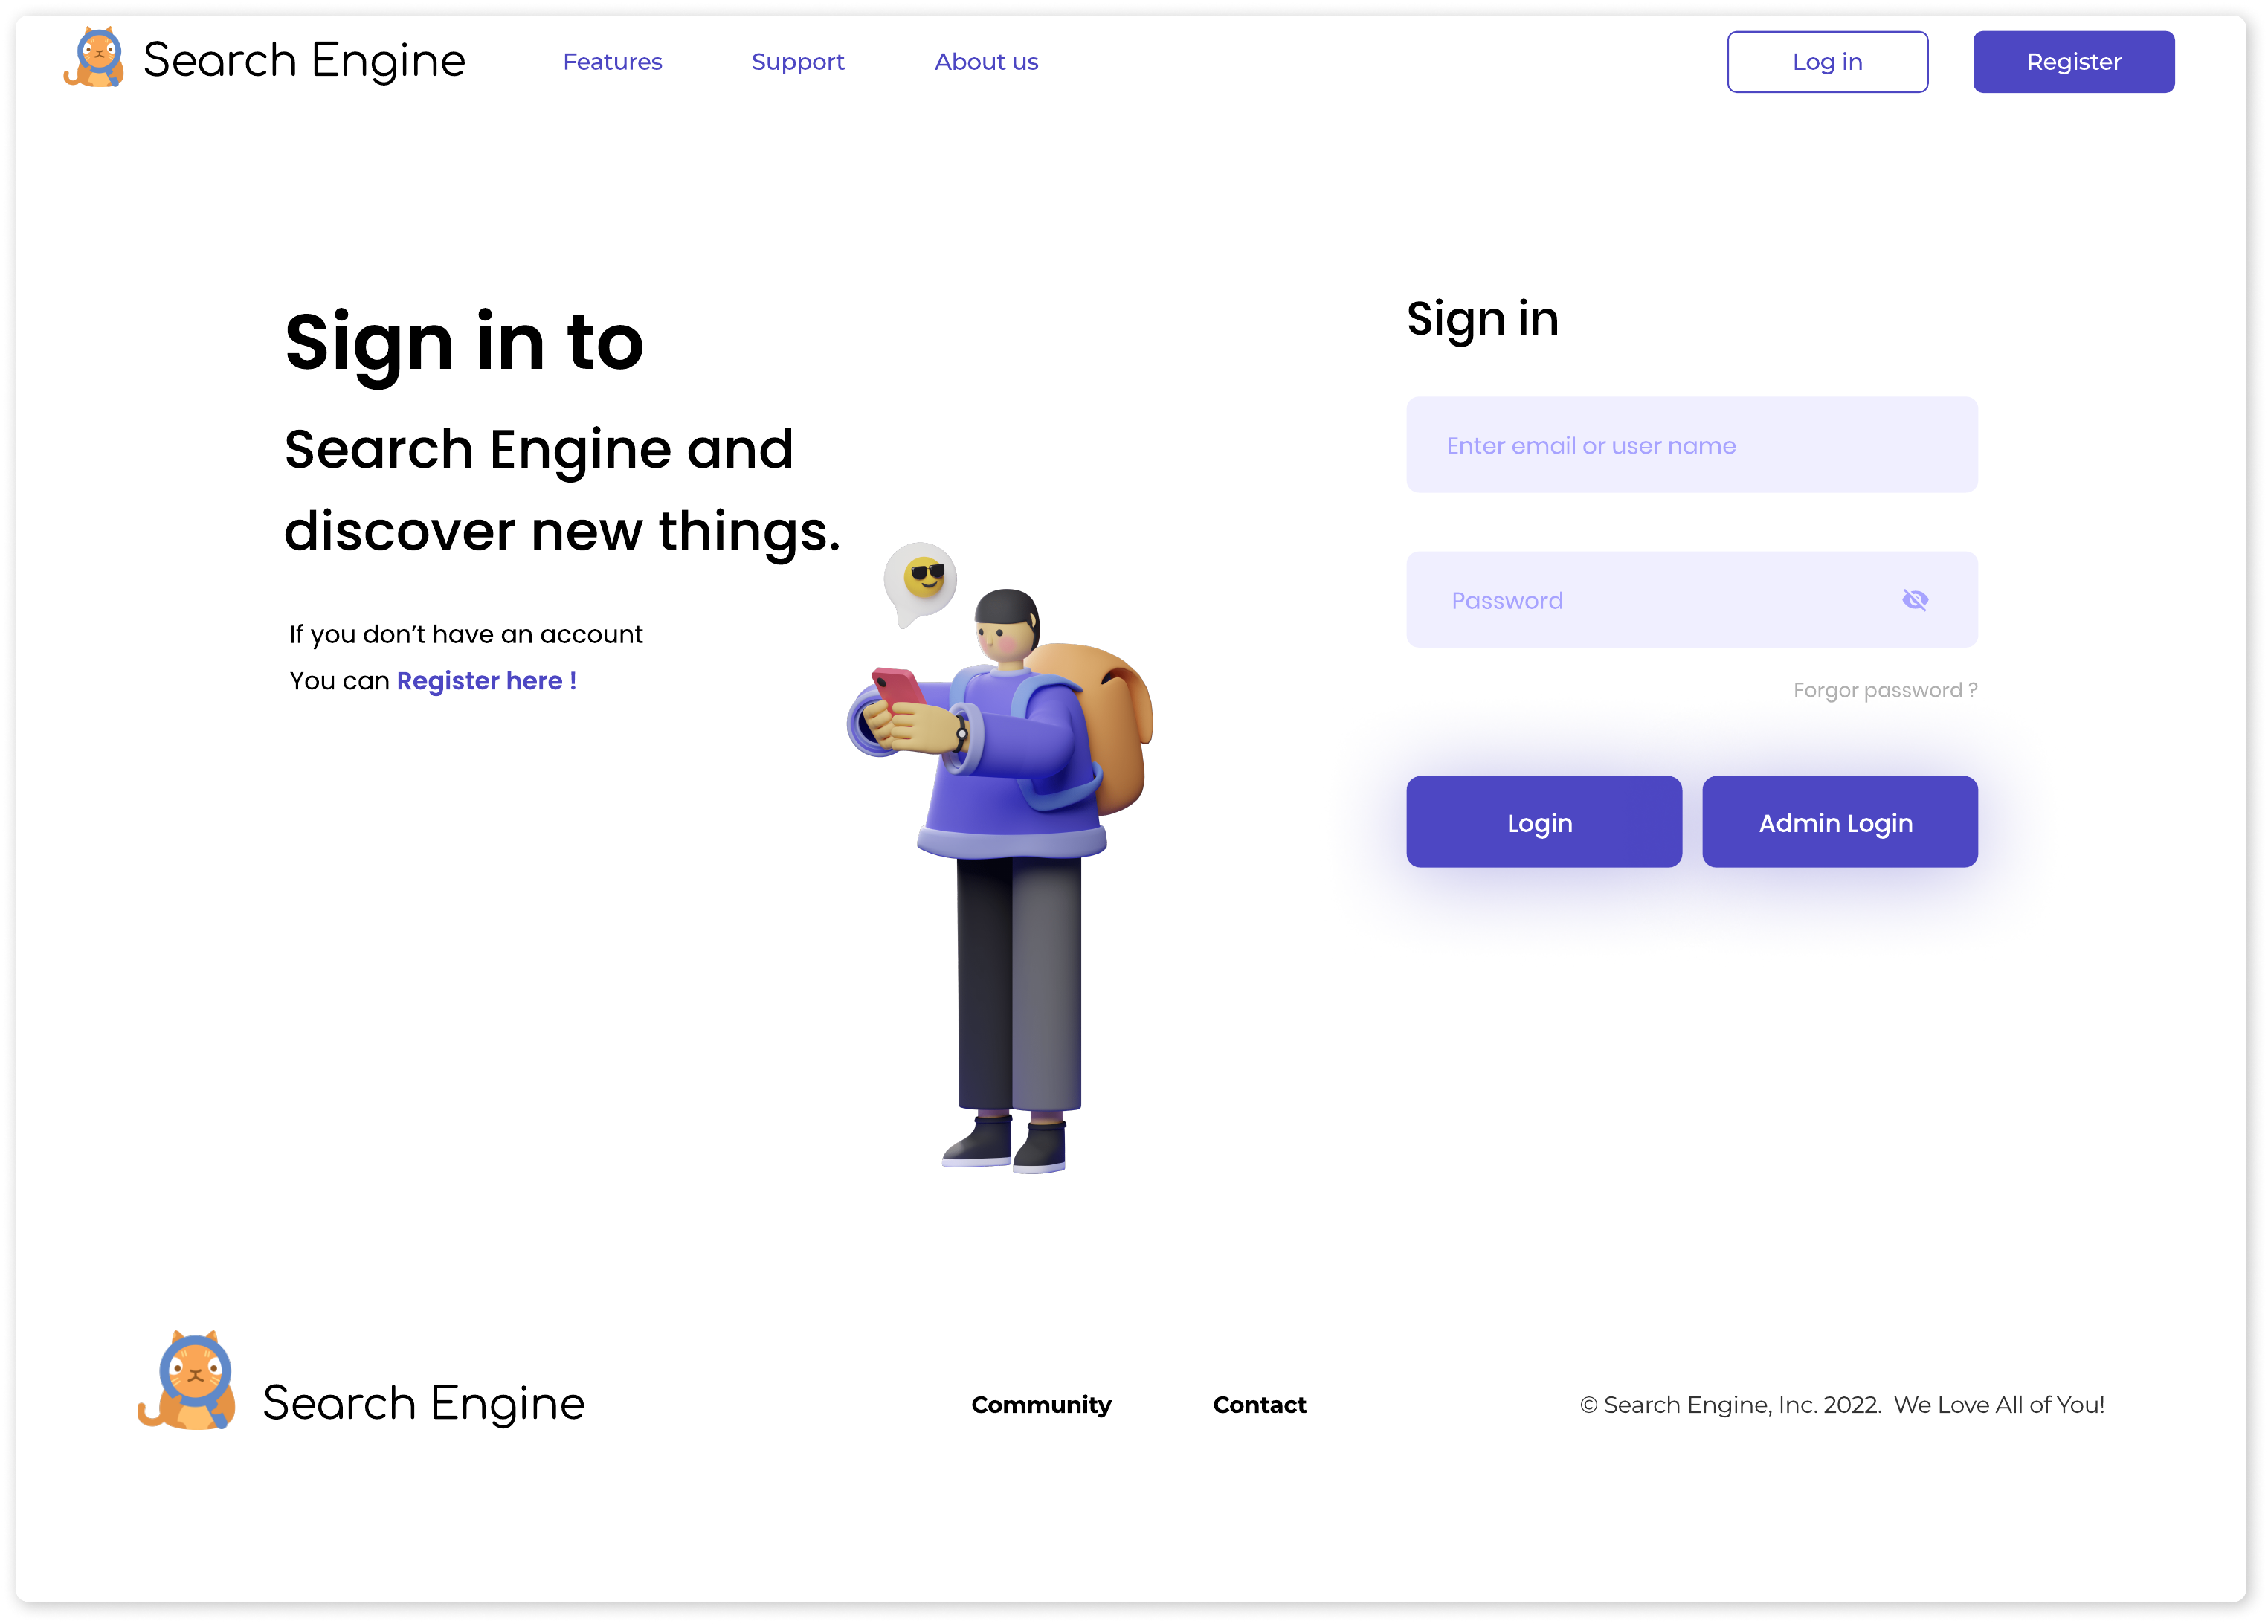
\includegraphics[scale=0.23]{login.pdf}
                       \end{center}
                       }
    \\\hline
    Pre Conditions & {
                     \begin{itemize}
                     \item US\_4
                     \end{itemize}
                     }\vspace*{-\baselineskip}
    \\\hline
    Acceptance Criteria & {
                          \begin{center}
                            \textbf{Senario: } User successfully login into the system. \\
                          \end{center}
    \textbf{Given} The user navigates to the login page, \textbf{When} The user enters a valid username and password \textbf{And} The user clicks on the Login button, \textbf{Then} The user will successfully login into the system.
    }
    \\\bottomrule
  \end{tabular}
\end{table}

\begin{table}[H]
  \caption{Search box, user story 6}
  \begin{tabular}{p{0.20\linewidth} | p{0.74\linewidth}}
    \toprule
    ID & US\_6
    \\\midrule
    Summary & \textbf{Search box}
    \\\hline
    Description & \textbf{As a} user, \textbf{I want} to be able to use the search box on the search page, \textbf{So that} I can be able to query.
    \\\hline
    Priority & \textcolor{red}{Highest}
    \\\hline
    Story Points & 8
    \\\hline
    UI/UX Attachment & {
                       \begin{center}
                         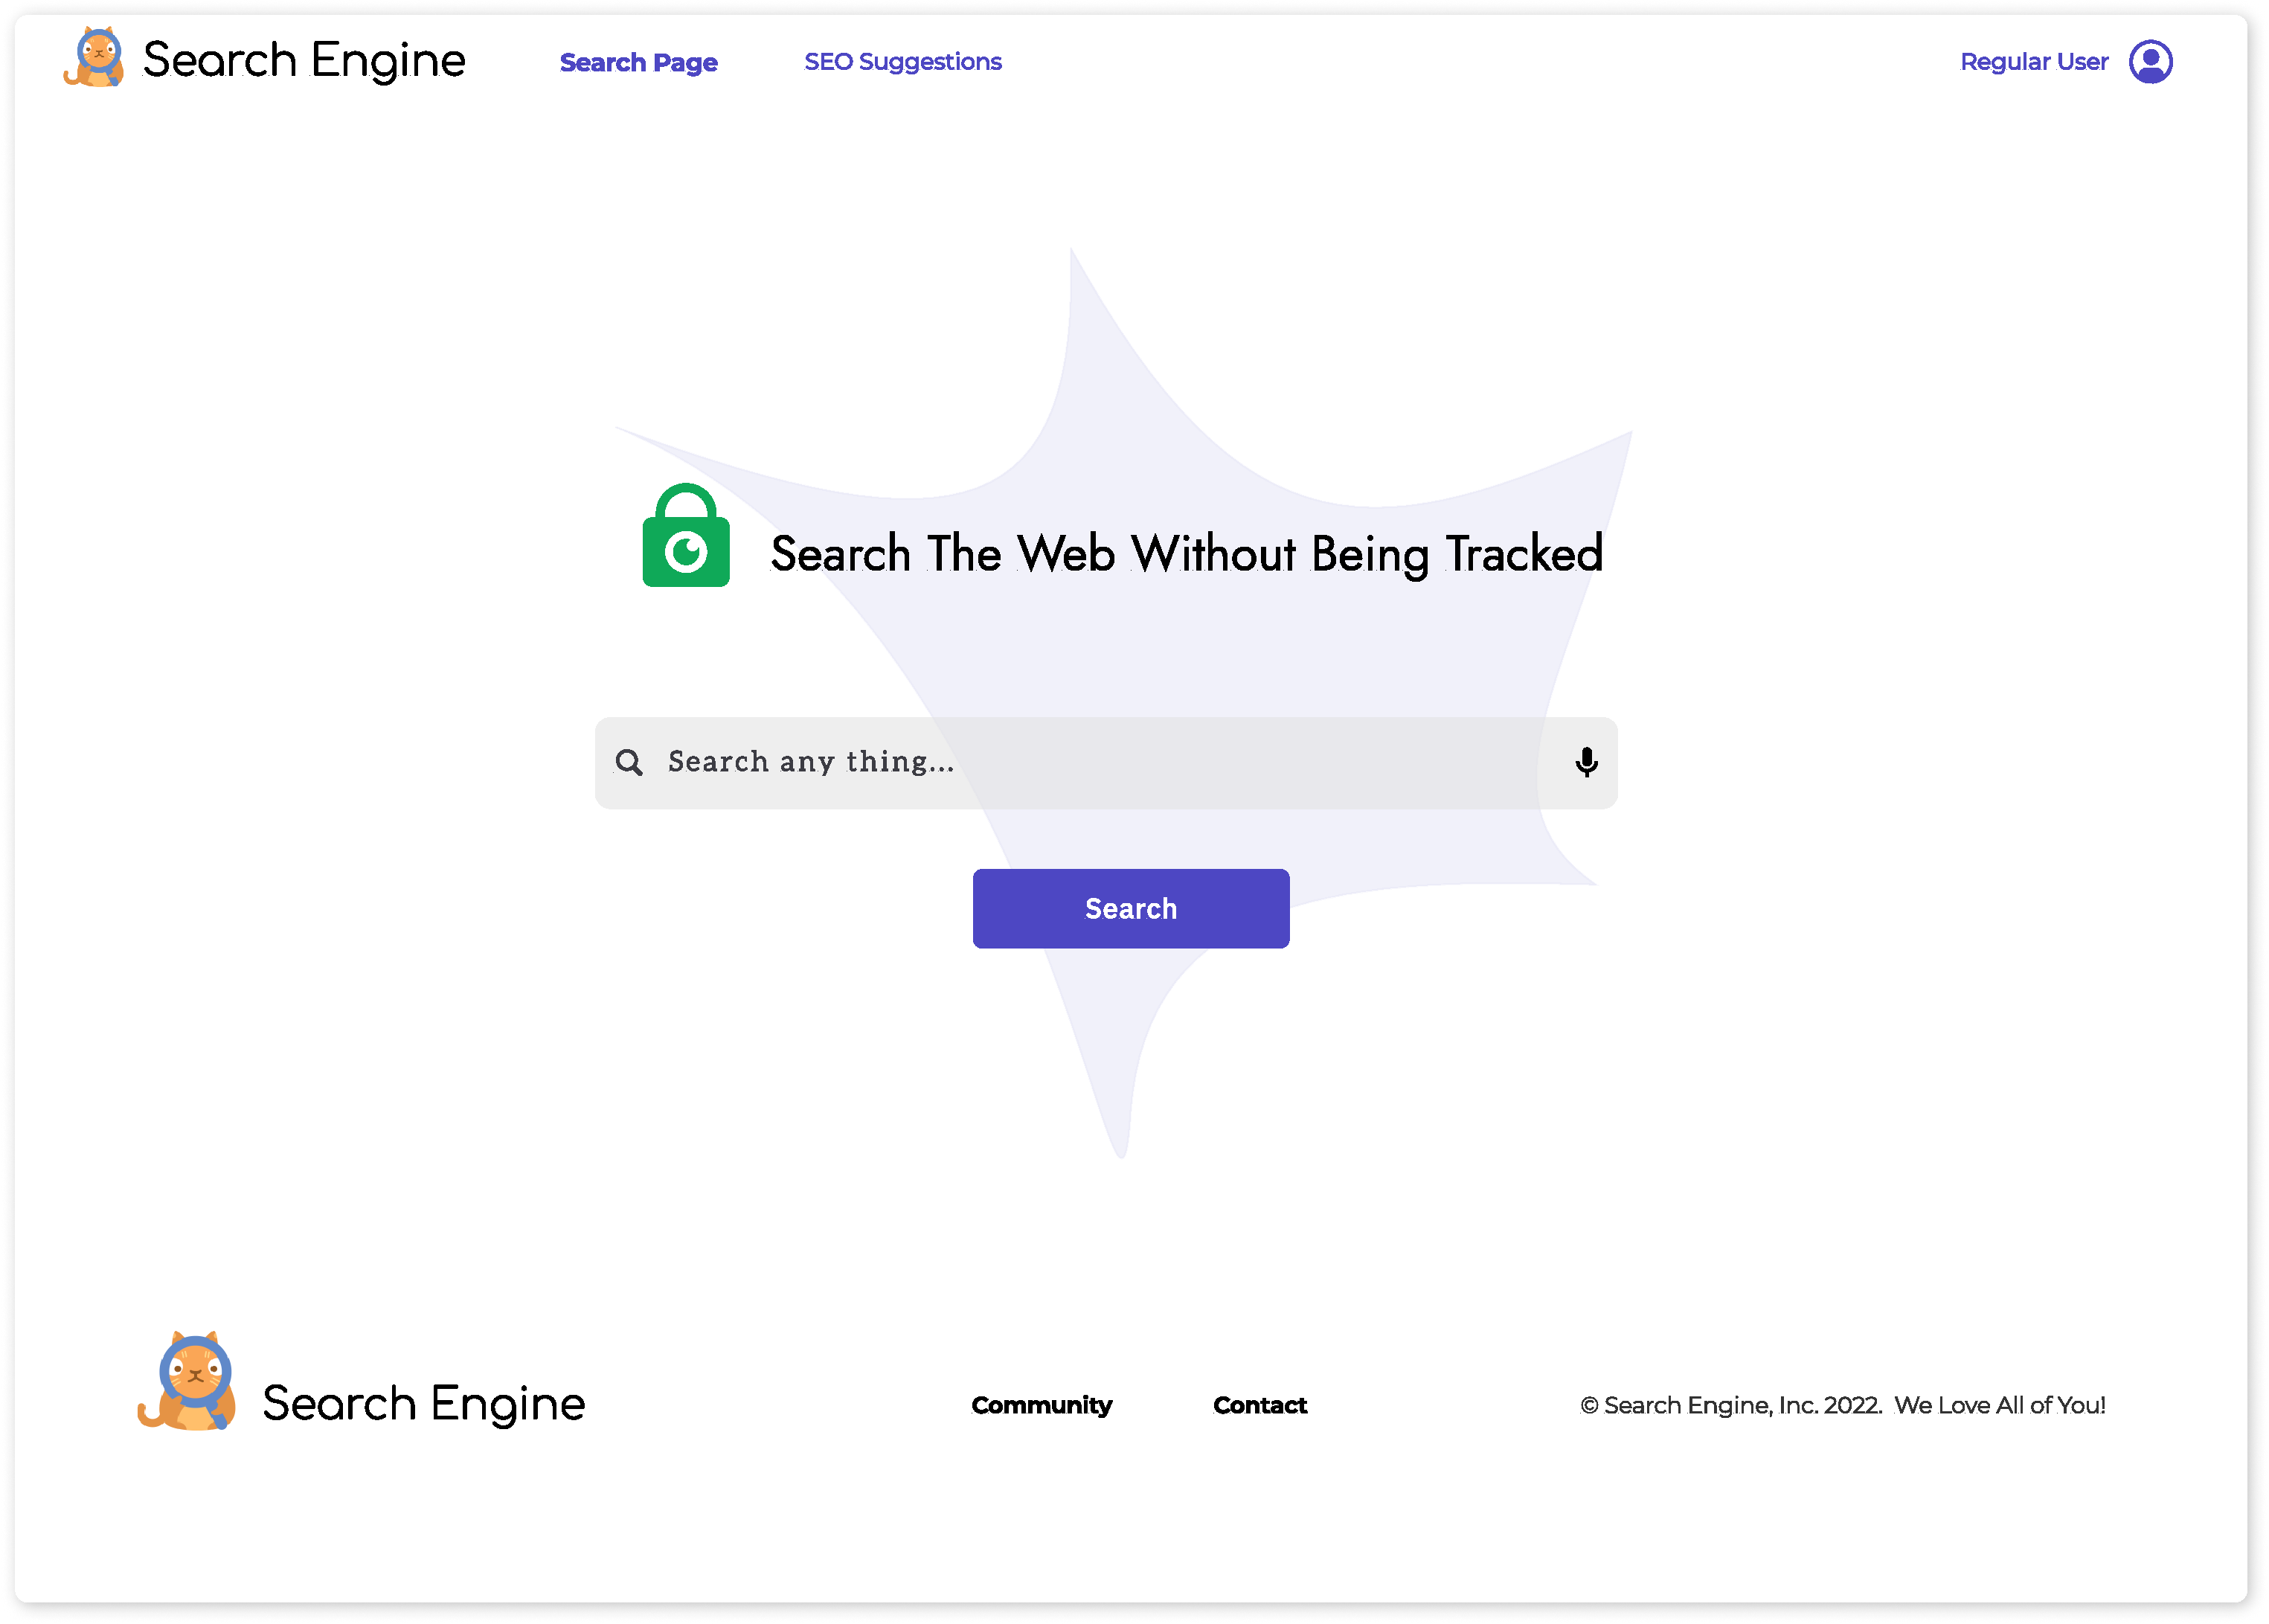
\includegraphics[scale=0.2]{search-box.pdf}
                         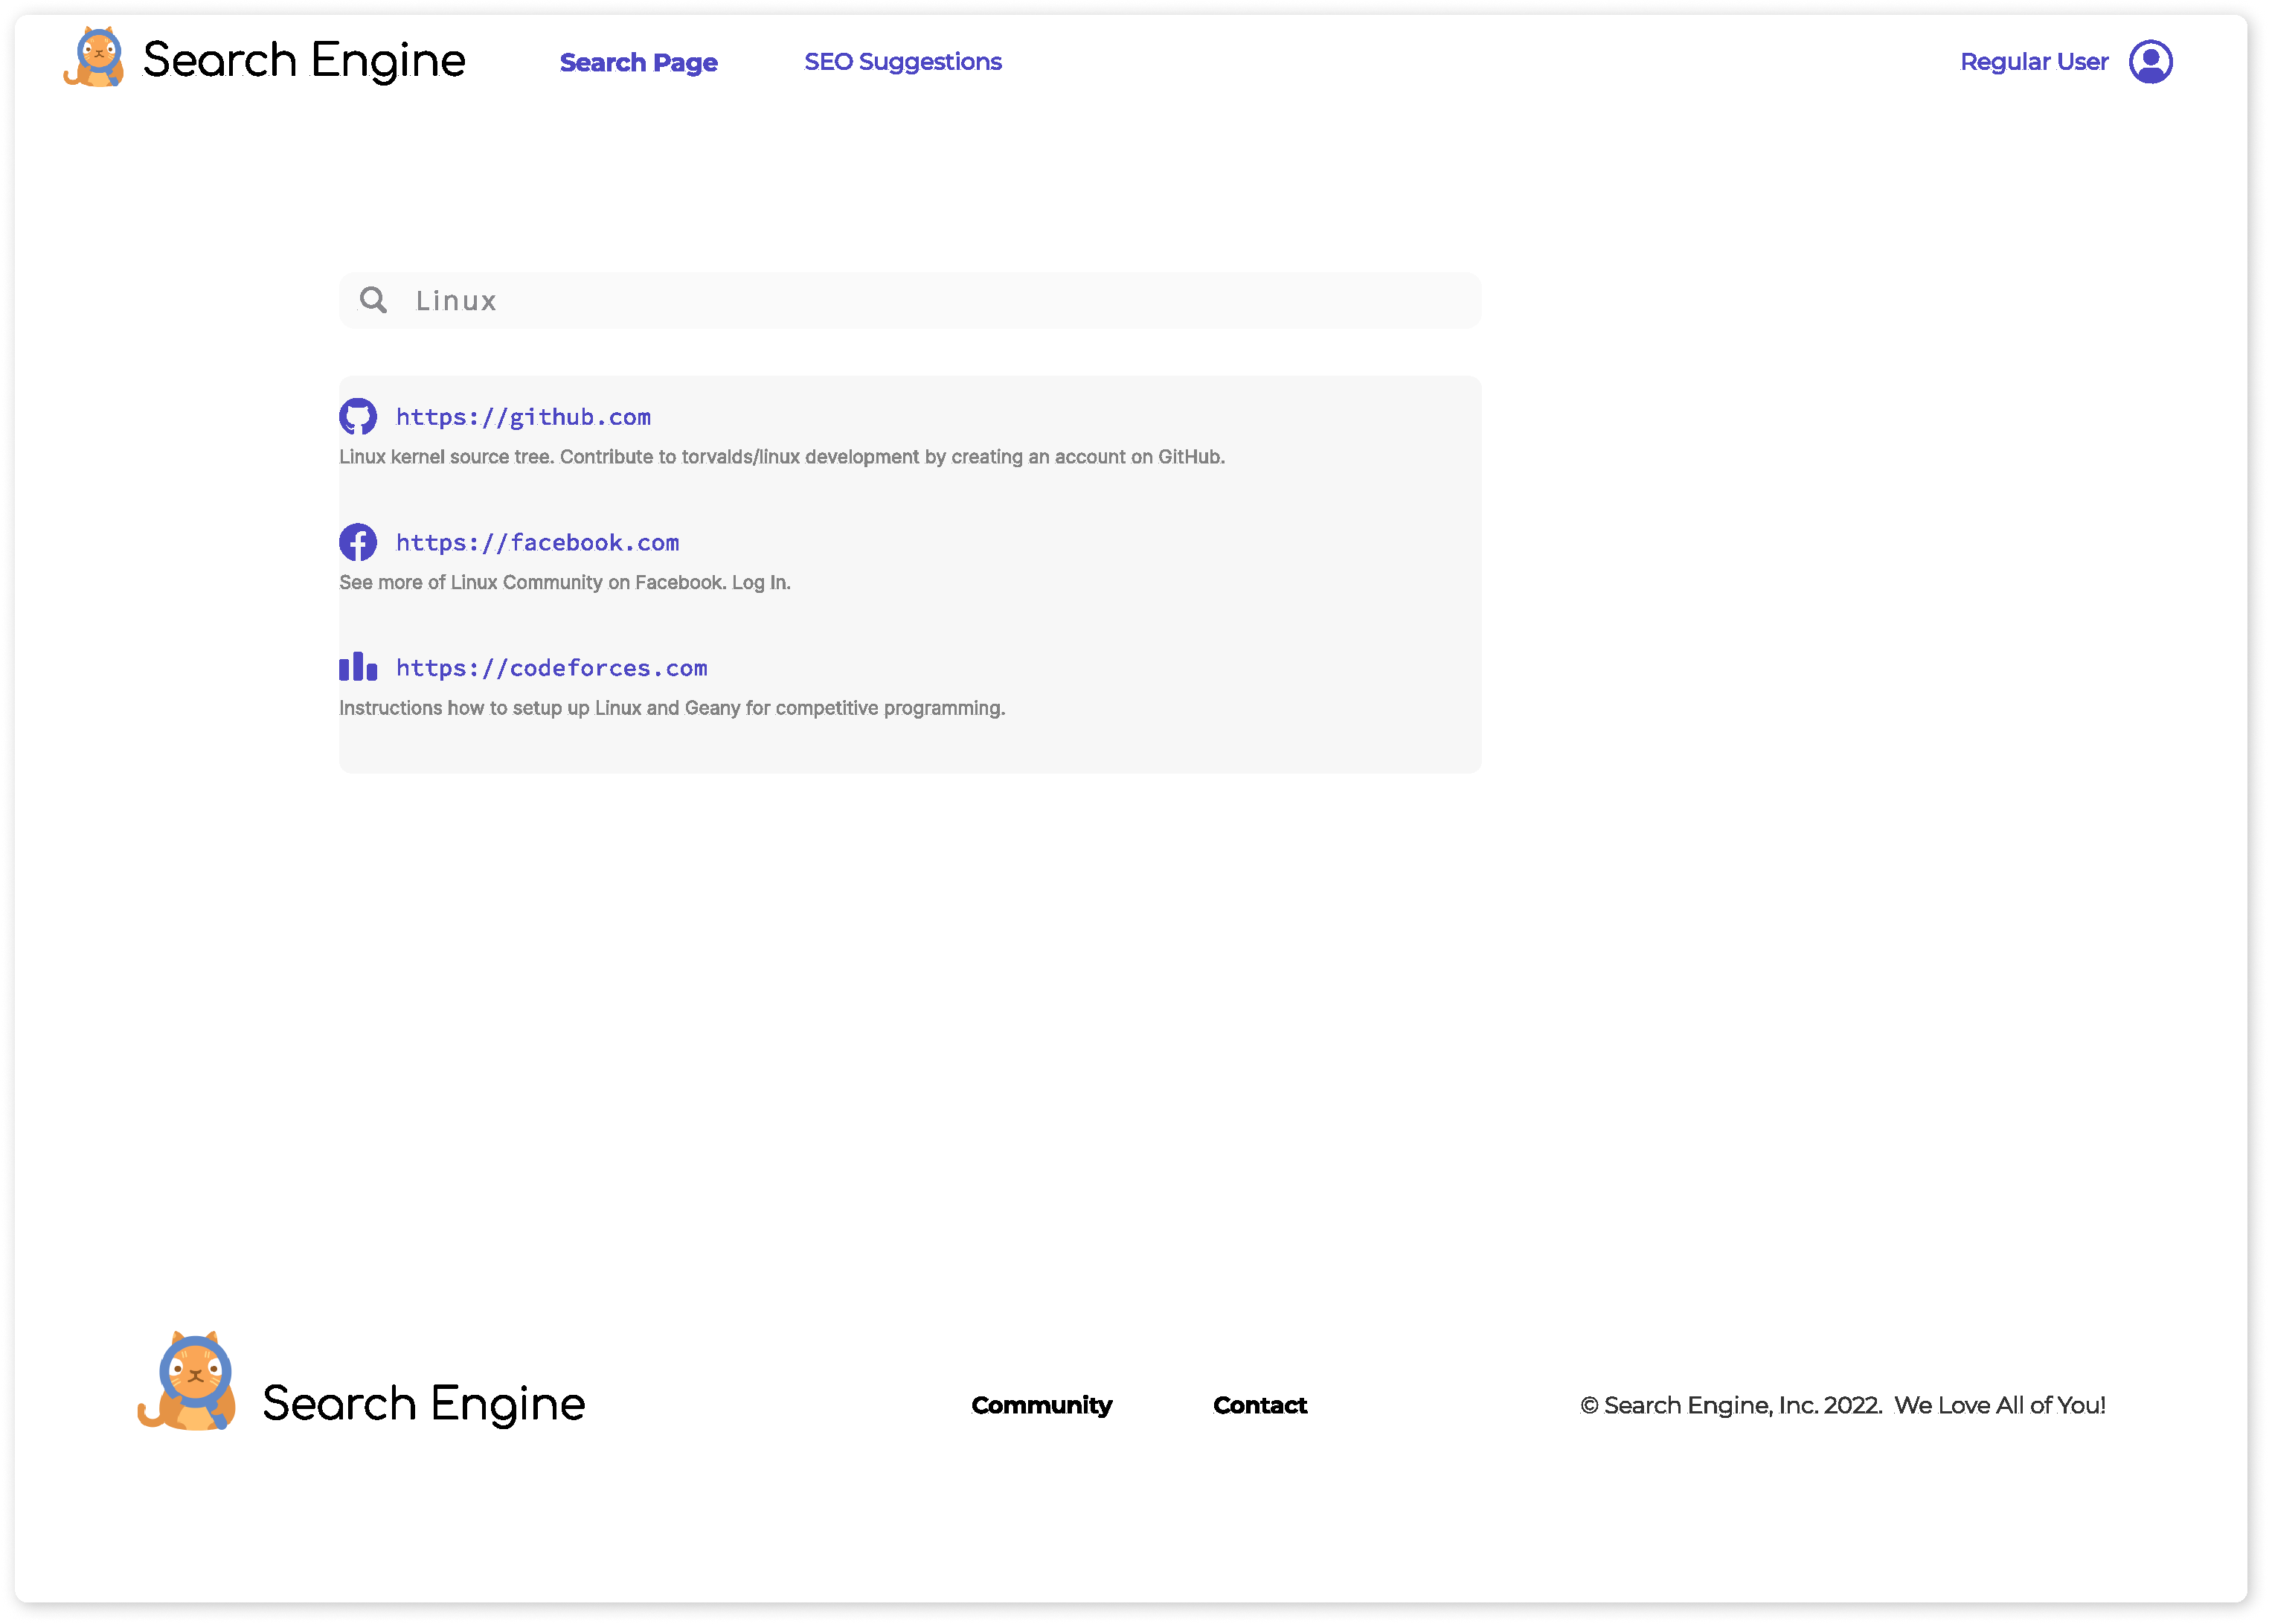
\includegraphics[scale=0.2]{search-result.pdf}
                       \end{center}
                       }
    \\\hline
    Pre Conditions & {
                     \begin{itemize}
                     \item US\_5
                     \end{itemize}
                     }\vspace*{-\baselineskip}
    \\\hline
    Acceptance Criteria & {
                          \begin{center}
                            \textbf{Senario: } User successfully using the search box. \\
                          \end{center}
    \textbf{Given} The user navigates to the search page, \textbf{When} The user enters a query in the search box \textbf{And} The user clicks on the Search button, \textbf{Then} The system will generate a list of website URLs related to that query.
    }
    \\\bottomrule
  \end{tabular}
\end{table}

\begin{table}[H]
  \caption{Keywords and meta-descriptions extraction, user story 7}
  \begin{tabular}{p{0.20\linewidth} | p{0.74\linewidth}}
    \toprule
    ID & US\_7
    \\\midrule
    Summary & \textbf{Keywords and meta-descriptions extraction}
    \\\hline
    Description & \textbf{As a} website owner, \textbf{I want} to search a live URL, \textbf{So that} I can get suitable keywords and meta-descriptions for my website.
    \\\hline
    Priority & \textcolor{magenta}{Medium}
    \\\hline
    Story Points & 5
    \\\hline
    UI/UX Attachment & {
                       \begin{center}
                         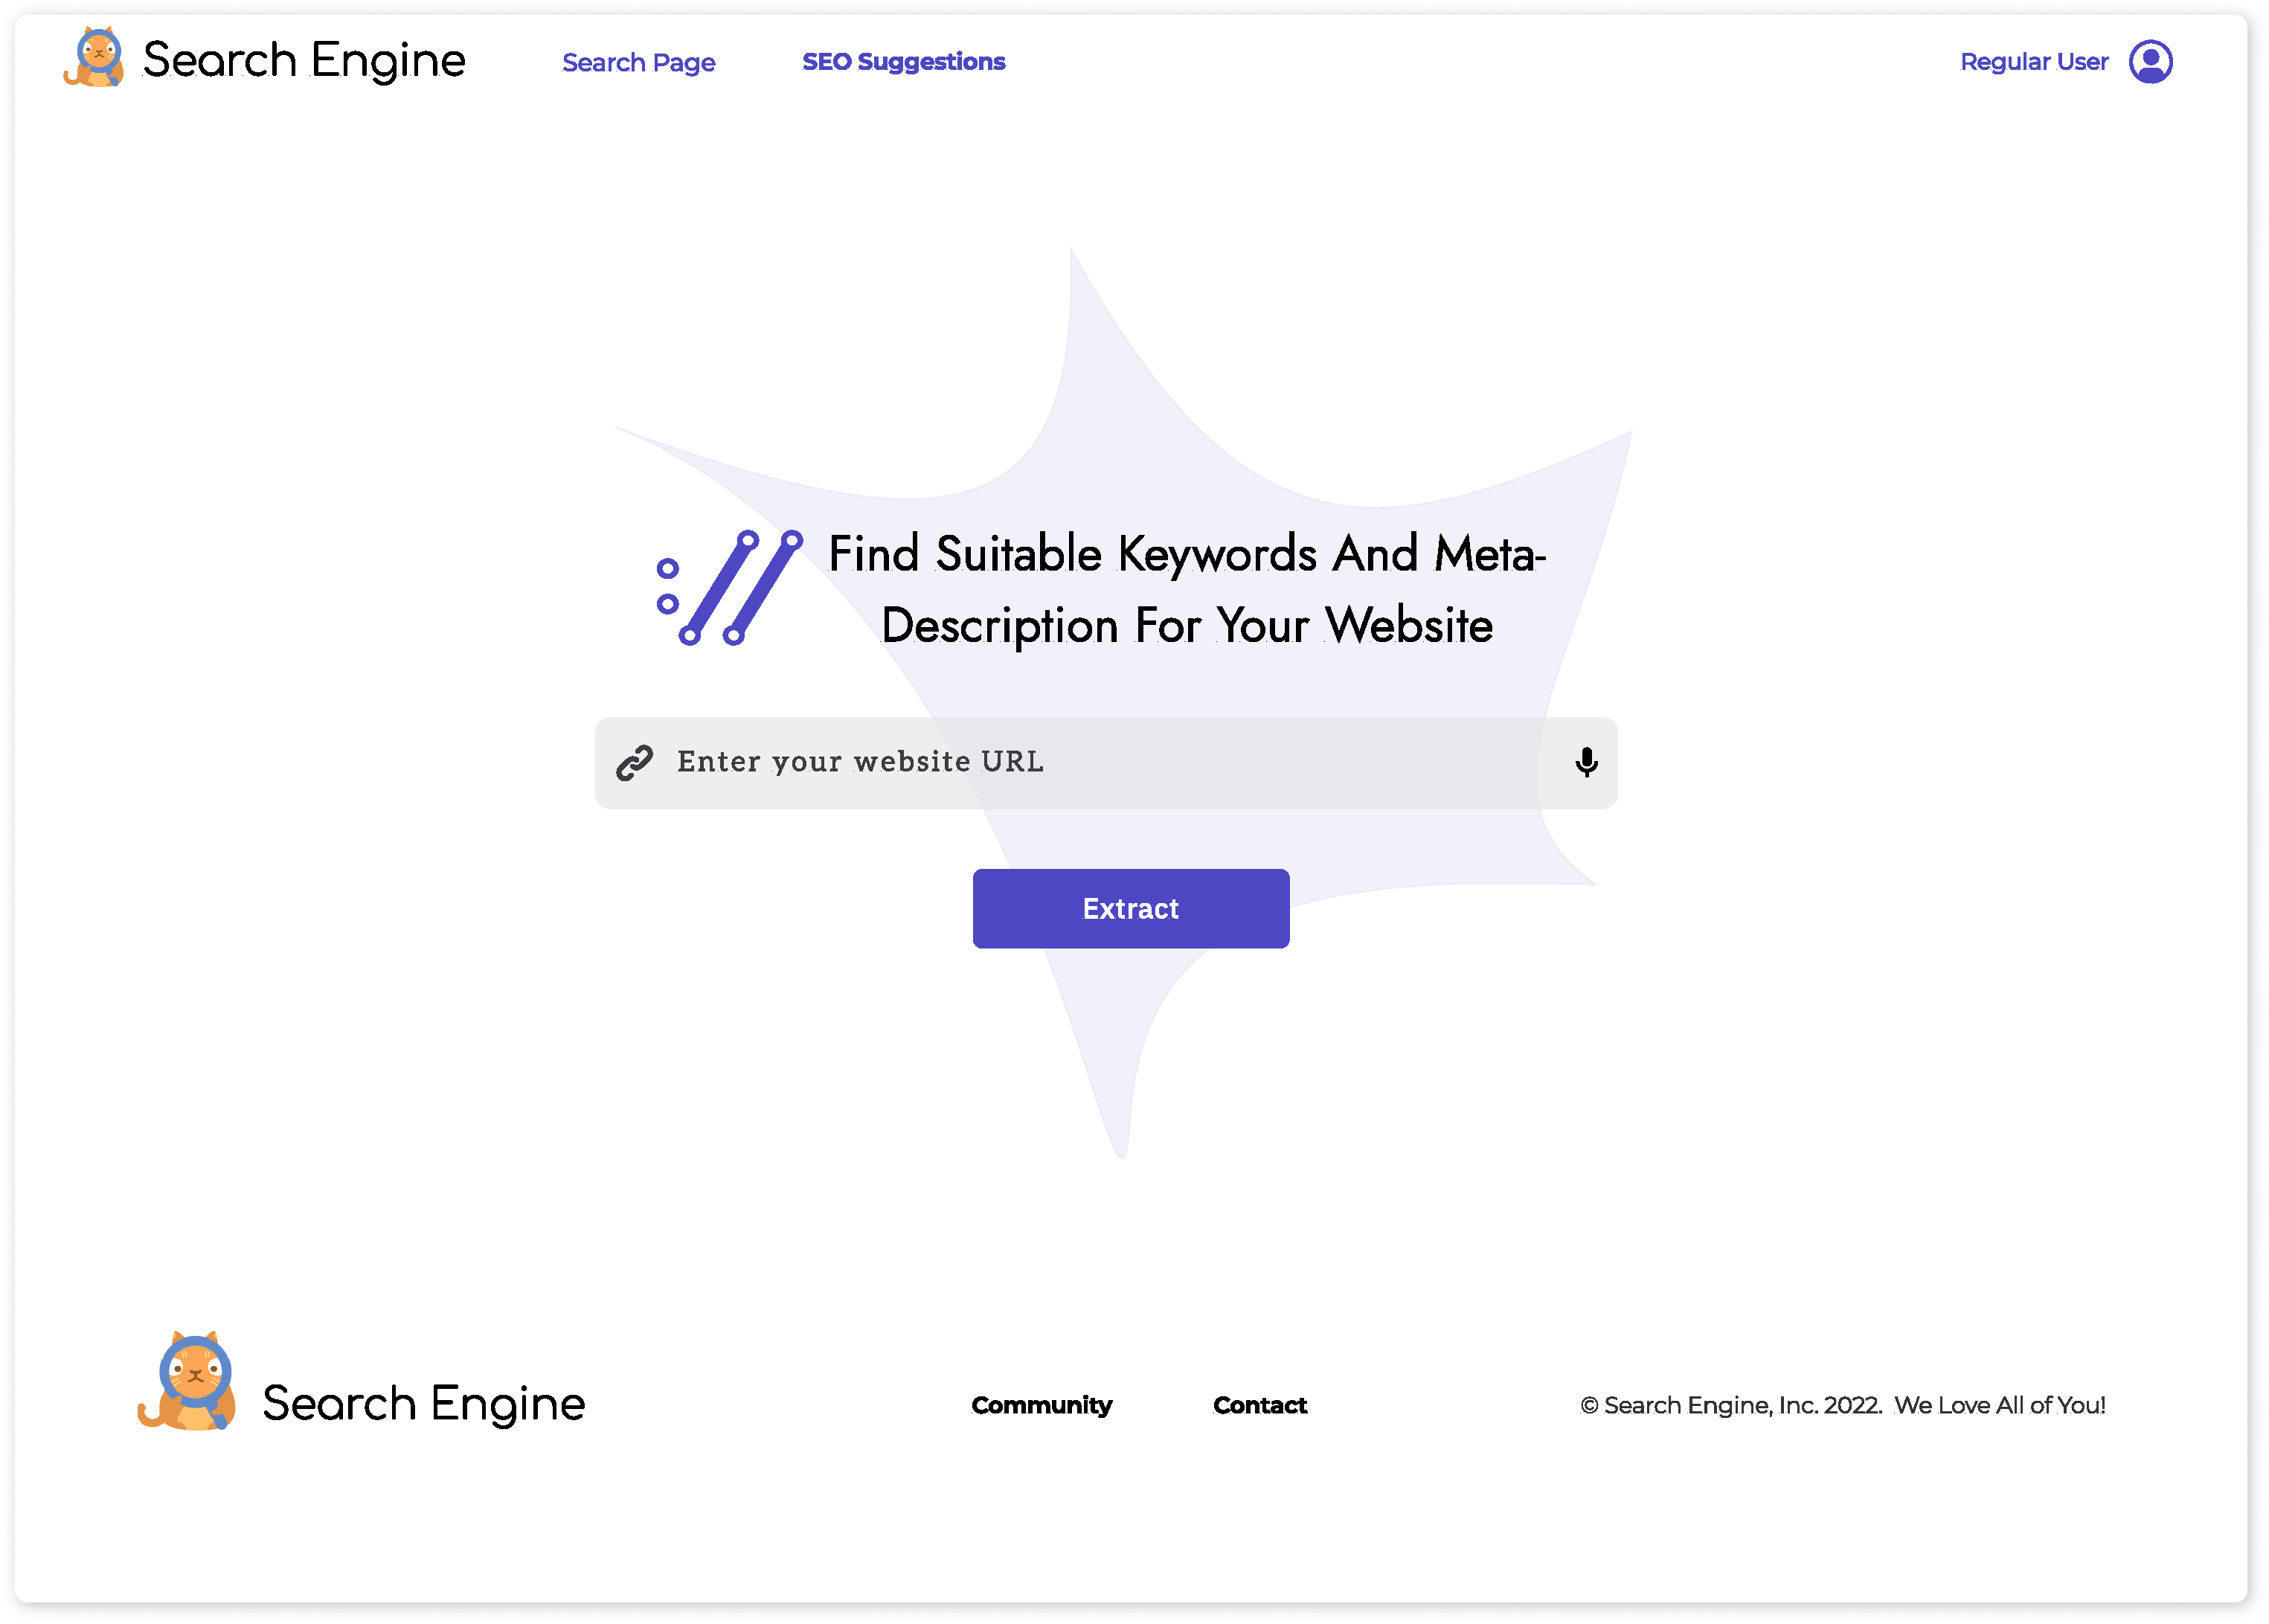
\includegraphics[scale=0.20]{seo-suggestions.pdf}
                         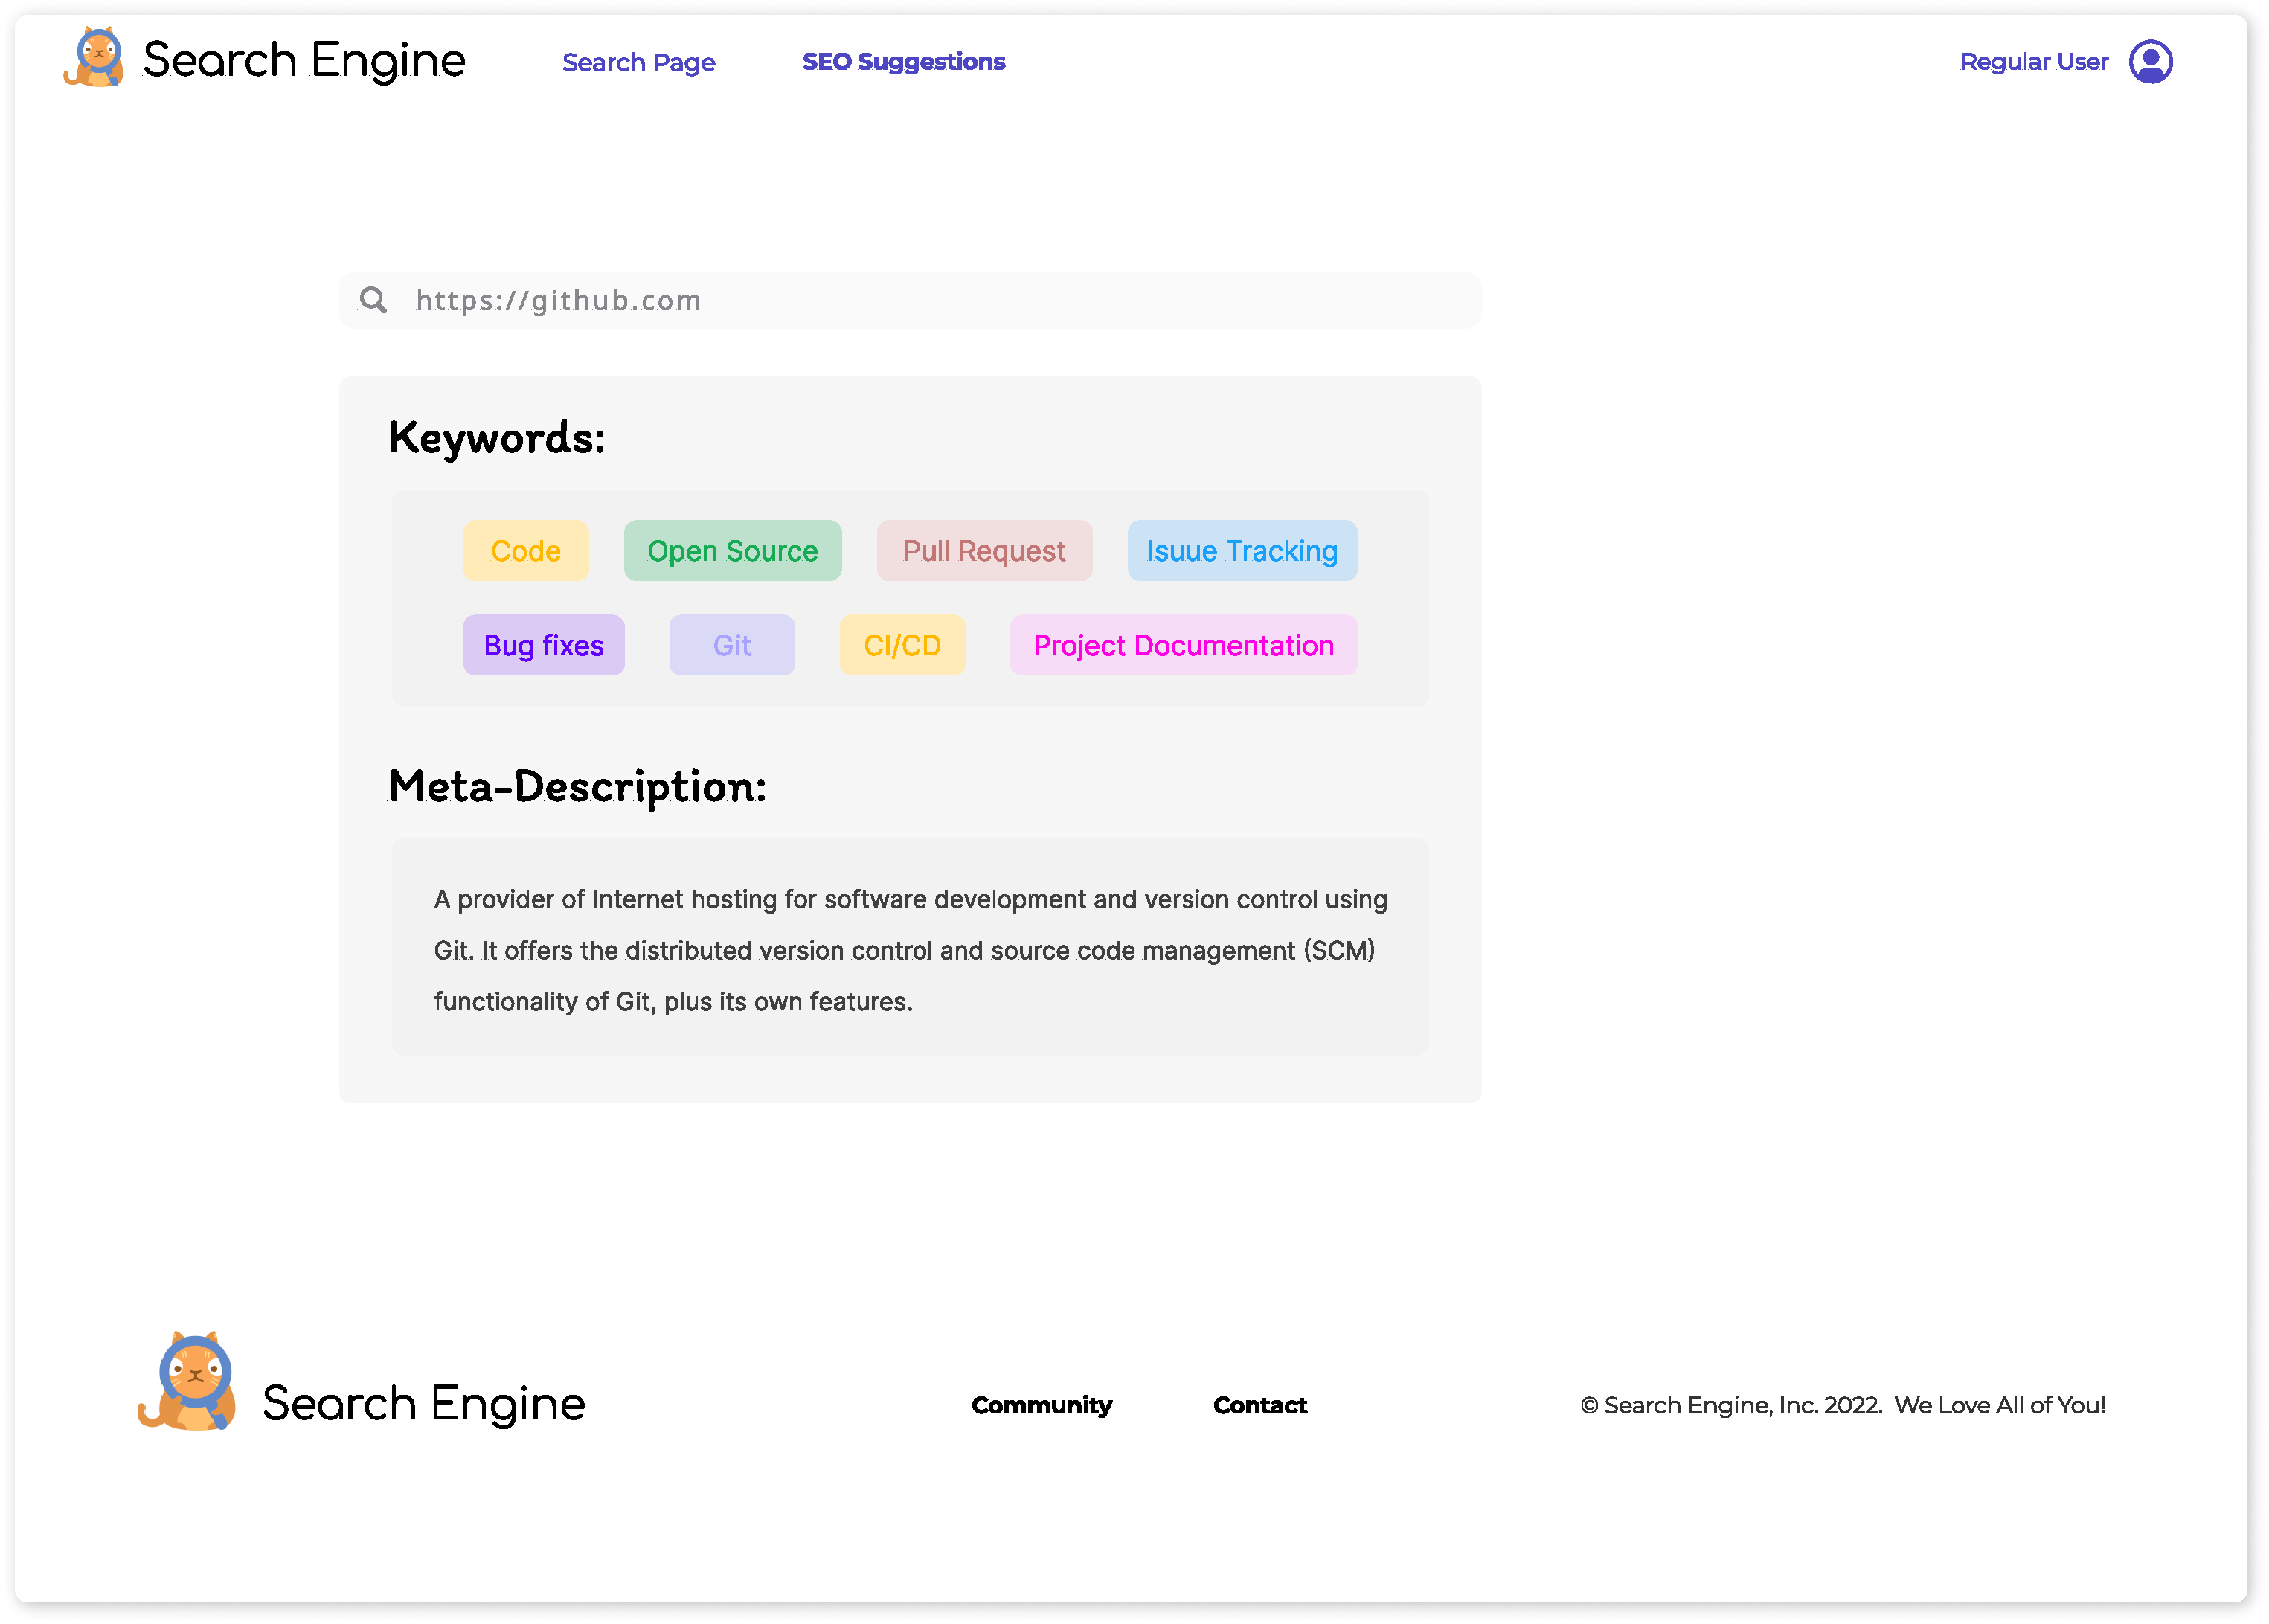
\includegraphics[scale=0.20]{seo-suggestions-result.pdf}
                       \end{center}
                       }
    \\\hline
    Pre Conditions & {
                     \begin{itemize}
                     \item US\_5
                     \end{itemize}
                     }\vspace*{-\baselineskip}
    \\\hline
    Acceptance Criteria & {
                          \begin{center}
                            \textbf{Senario: } Website owner successfully using the live URL search box for extracting keywords. \\
                          \end{center}
    \textbf{Given} The website owner navigates to the seo suggestions page, \textbf{When} The website owner enters a live URL in the search box \textbf{And} The website owner clicks on the Extract button, \textbf{Then} The system will generate a list of keywords and meta-descriptions from that website's data.
    }
    \\\bottomrule
  \end{tabular}
\end{table}

\section{Use Cases}

\subsection{Use Case Diagram}

The diagram below visualizes all the actors in the system and all the interactions each actor can do.

\begin{figure}[H]
  \begin{center}
    \caption{User case diagram}
    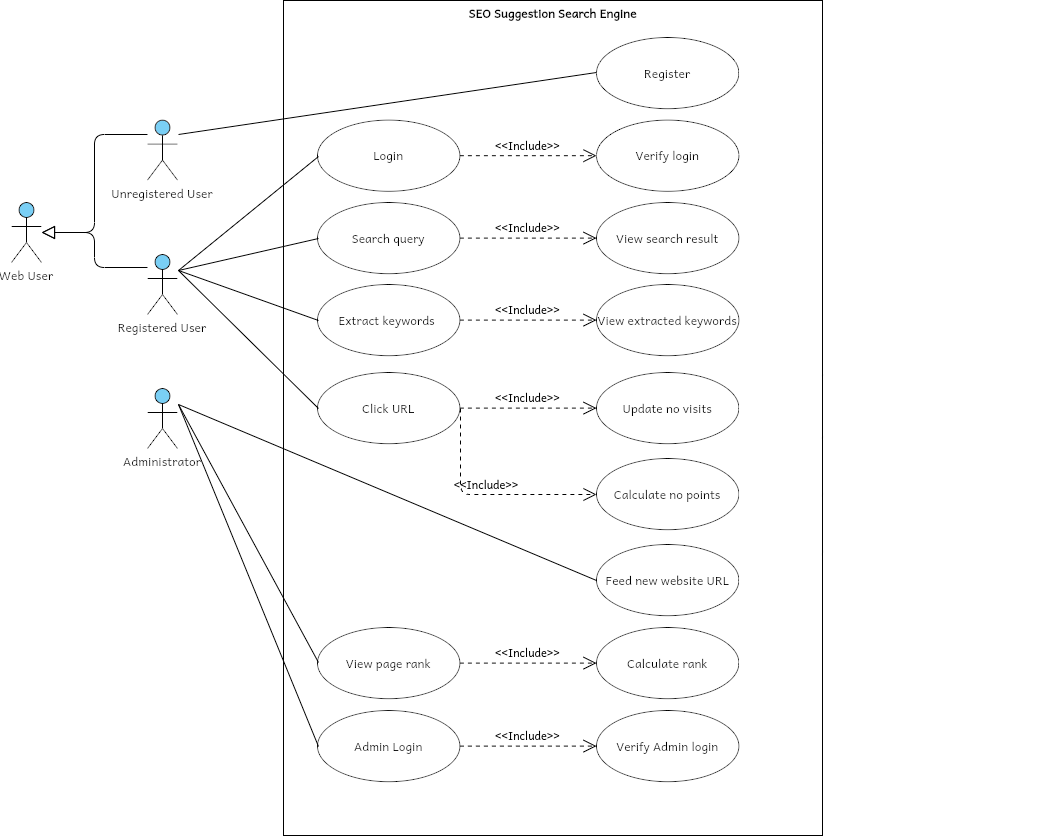
\includegraphics[scale=0.44]{use-cases-diagram.png}
  \end{center}
\end{figure}

\newpage

\subsection{Use Case Model}

This section includes the details, description, and the main success scenario of use cases in an organized way.

\begin{table}[H]
  \caption{Administrator login, use case 1}
  \begin{tabular}{p{0.20\linewidth} | p{0.74\linewidth}}
    \toprule
    ID & UC\_1
    \\\midrule
    Title & \textbf{Administrator login}
    \\\hline
    Description & The administrator shall login into the system using admin credentials.
    \\\hline
    Primary Actor & Administrator
    \\\hline
    Pre-Conditions & {
                     \begin{itemize}
                     \item The administrator should have the authorization credentials to enter the admin area.
                     \end{itemize}
                     }\vspace*{-\baselineskip}
    \\\hline
    Post-Conditions & -
    \\\hline
    Main Success Scenario & {
                            \begin{enumerate}
                            \item The administrator fills in username and password fields.
                            \item The administrator clicks on the admin login button.
                            \item The system will validate the username and password. If correct, login into the system; otherwise, stay on the current login page.
                            \end{enumerate}
                            }\vspace*{-\baselineskip}
    \\\bottomrule
  \end{tabular}
\end{table}

\begin{table}[H]
  \caption{Feed new website URL, use case 2}
  \begin{tabular}{p{0.20\linewidth} | p{0.74\linewidth}}
    \toprule
    ID & UC\_2
    \\\midrule
    Title & \textbf{Feed new website URL}
    \\\hline
    Description & The administrator shall feed a new website URL and its metadata into the system.
    \\\hline
    Primary Actor & Administrator
    \\\hline
    Pre Conditions & {
                     \begin{itemize}
                     \item UC\_1
                     \end{itemize}
                     }\vspace*{-\baselineskip}
    \\\hline
    Post Conditions & The system saves the data to the database.
    \\\hline
    Main Success Scenario & {
                            \begin{enumerate}
                            \item The administrator feeds the database website URLs and its metadata.
                            \item The administrator clicks on add new website button.
                            \item The system saves the data in a new row in the database.
                            \end{enumerate}
                            }\vspace*{-\baselineskip}
    \\\bottomrule
  \end{tabular}
\end{table}

\begin{table}[H]
  \caption{View page rank calculations, use case 3}
  \begin{tabular}{p{0.20\linewidth} | p{0.74\linewidth}}
    \toprule
    ID & UC\_3
    \\\midrule
    Title & \textbf{View page rank calculations}
    \\\hline
    Description & The administrator shall be able to view the page rank calculations.
    \\\hline
    Primary Actor & Administrator
    \\\hline
    Pre Conditions & {
                     \begin{itemize}
                     \item UC\_1
                     \end{itemize}
                     }\vspace*{-\baselineskip}
    \\\hline
    Post Conditions & -
    \\\hline
    Main Success Scenario & {
                            \begin{enumerate}
                            \item The administrator clicks the page ranking anchor in the tab menu.
                            \item The system lists the website URLs in the database sorted based on their number of visits and points.
                            \end{enumerate}
                            }\vspace*{-\baselineskip}
    \\\bottomrule
  \end{tabular}
\end{table}

\begin{table}[H]
  \caption{User registration, use case 4}
  \begin{tabular}{p{0.20\linewidth} | p{0.74\linewidth}}
    \toprule
    ID & UC\_4
    \\\midrule
    Title & \textbf{User registration}
    \\\hline
    Description & The user shall be able to register to the system.
    \\\hline
    Primary Actor & User
    \\\hline
    Pre Conditions & -
    \\\hline
    Post Conditions & The system redirects the user to the login page.
    \\\hline
    Main Success Scenario & {
                            \begin{enumerate}
                            \item The user enters a valid email, password, username, full name, and confirm the password correctly.
                            \item The user clicks the Sign up button.
                            \item The system successfully register the user into the system.
                            \end{enumerate}
                            }\vspace*{-\baselineskip}
    \\\bottomrule
  \end{tabular}
\end{table}

\begin{table}[H]
  \caption{User login, use case 5}
  \begin{tabular}{p{0.20\linewidth} | p{0.74\linewidth}}
    \toprule
    ID & UC\_5
    \\\midrule
    Title & \textbf{User login}
    \\\hline
    Description & The user shall be able to login into the system.
    \\\hline
    Primary Actor & User
    \\\hline
    Pre Conditions & {
                     \begin{itemize}
                     \item UC\_4
                     \end{itemize}
                     }\vspace*{-\baselineskip}
    \\\hline
    Post Conditions & The system redirects the user to the search page.
    \\\hline
    Main Success Scenario & {
                            \begin{enumerate}
                            \item The user fills in username and password fields.
                            \item The user clicks on the login button.
                            \item The system will validate the username and password. If correct, login; otherwise, stay on the current login page.
                            \end{enumerate}
                            }\vspace*{-\baselineskip}
    \\\bottomrule
  \end{tabular}
\end{table}

\begin{table}[H]
  \caption{Search query, use case 6}
  \begin{tabular}{p{0.20\linewidth} | p{0.74\linewidth}}
    \toprule
    ID & UC\_6
    \\\midrule
    Title & \textbf{Search query}
    \\\hline
    Description & The user shall be able to use the search functionality for searching specific terms.
    \\\hline
    Primary Actor & User
    \\\hline
    Pre Conditions & {
                     \begin{itemize}
                     \item UC\_5
                     \end{itemize}
                     }\vspace*{-\baselineskip}
    \\\hline
    Post Conditions & The system will generate a list of related website URLs that matches the query.
    \\\hline
    Main Success Scenario & {
                            \begin{enumerate}
                            \item The user clicks the search page anchor in the tab menu.
                            \item The system opens the page of the search.
                            \item The user write down his/her search query in the search box.
                            \item The user clicks the search button.
                            \item The system uses this query and matches it with the content provided in URLs fed in the database.
                            \item The system generates a list of related URLs.
                            \item The user can then click on any URL in the generated list, and the URL will open the corresponding website.
                            \item The system increases the number of visits to that URL in the database.
                            \item The system goes to the web page URL to fetch its metadata and gives points according to page errors.
                            \item The system updates the page's rank in the database according to the points the page gains and the number of visits.
                            \end{enumerate}
                            }\vspace*{-\baselineskip}
    \\\bottomrule
  \end{tabular}
\end{table}

\begin{table}[H]
  \caption{Extract keywords and meta-descriptions, use case 7}
  \begin{tabular}{p{0.20\linewidth} | p{0.74\linewidth}}
    \toprule
    ID & UC\_7
    \\\midrule
    Title & \textbf{Extract keywords and meta-descriptions}
    \\\hline
    Description & The website owner shall be able to use the SEO suggestion to find suitable keywords and meta-descriptions for their website.
    \\\hline
    Primary Actor & User
    \\\hline
    Pre Conditions & {
                     \begin{itemize}
                     \item UC\_5
                     \end{itemize}
                     }\vspace*{-\baselineskip}
    \\\hline
    Post Conditions & The system will extract a list of keywords and meta-descriptions from that particular URL.
    \\\hline
    Main Success Scenario & {
                            \begin{enumerate}
                            \item The user write down a live URL in the search box.
                            \item The user clicks the find keywords and meta-description button.
                            \item The system goes and scans the web page URL, extracts its meta-features.
                            \item The system then lists out suitable keywords related to the contents of the web page URL and a meta-description.
                            \end{enumerate}
                            }\vspace*{-\baselineskip}
    \\\bottomrule
  \end{tabular}
\end{table}

\section{Sequence Diagram}

The sequence diagrams below show the interactions between the system with each other.

\begin{figure}[H]
  \begin{center}
    \caption{Administrator login, sequence diagram 1}
    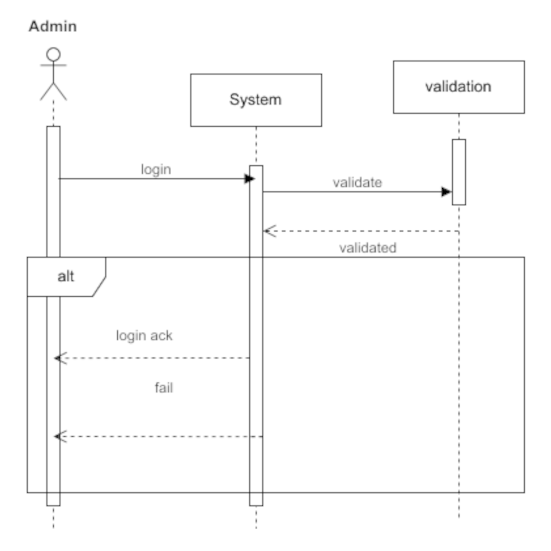
\includegraphics[scale=0.63]{seq-diagram-1.png}
  \end{center}
\end{figure}

\begin{figure}[H]
  \begin{center}
    \caption{Feeds new website URL, sequence diagram 2}
    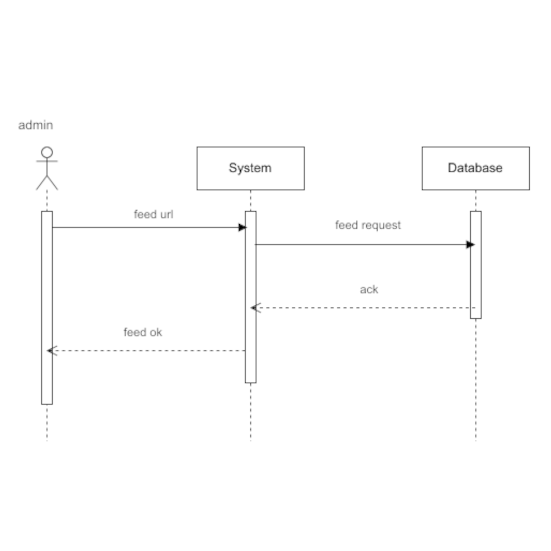
\includegraphics[scale=0.7]{seq-diagram-2.png}
  \end{center}
\end{figure}

\begin{figure}[H]
  \begin{center}
    \caption{Search query, sequence diagram 3}
    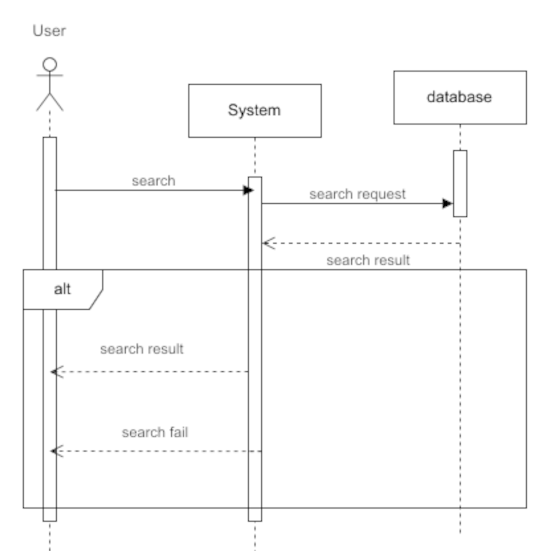
\includegraphics[scale=0.65]{seq-diagram-3.png}
  \end{center}
\end{figure}

\begin{figure}[H]
  \begin{center}
    \caption{Clicks URL, sequence diagram 4}
    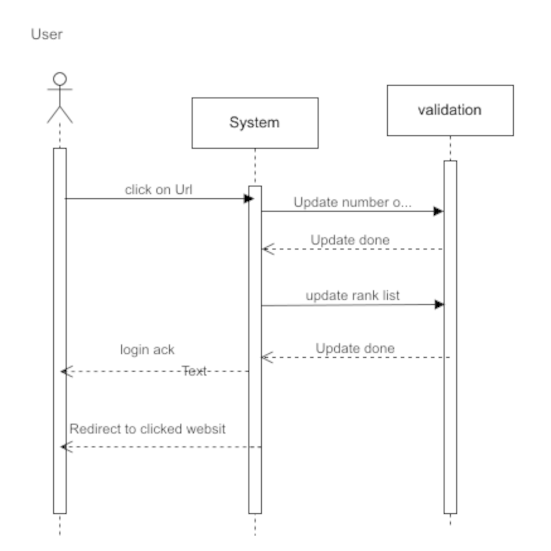
\includegraphics[scale=0.7]{seq-diagram-4.png}
  \end{center}
\end{figure}

\begin{figure}[H]
  \begin{center}
    \caption{SEO Suggestions, sequence diagram 5}
    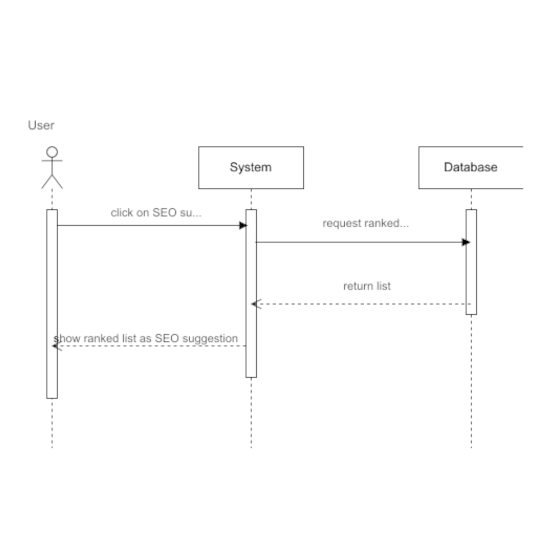
\includegraphics[scale=0.72]{seq-diagram-5.png}
  \end{center}
\end{figure}

\newpage

\section{Entity Relationship Diagram}

The following diagram below shows the relationship between the system entities.

\begin{figure}[H]
  \begin{center}
    \caption{Entity relationship diagram}
    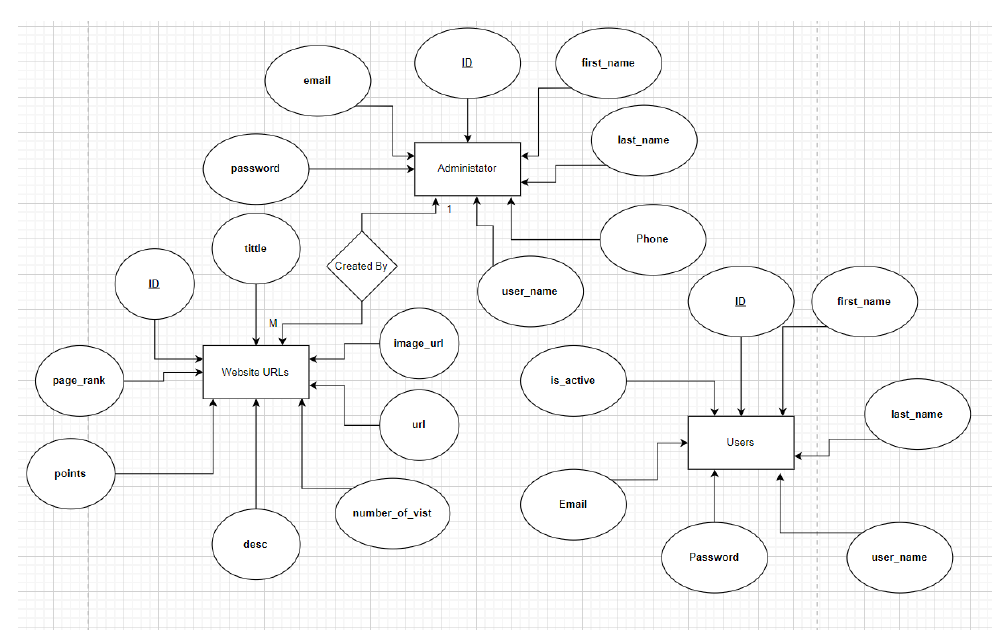
\includegraphics[scale=0.95]{erd-diagram.png}
  \end{center}
\end{figure}

\section{Test Scripts}

Below are the test scripts for checking if the application acts as expected.

\begin{table}[H]
  \caption{Check admin login with valid credentials, test case 1}
  \begin{tabular}{p{0.2\linewidth} | p{0.74\linewidth}}
    \toprule
    ID & TC\_1
    \\\midrule
    Description & Check Admin login with valid credentials
    \\\hline
    Priority & \textcolor{orange}{High}
    \\\hline
    Test Steps & {
                 \begin{enumerate}
                 \item Go to \url{https://search-engine.org/login}
                 \item Enter Username
                 \item Enter Password
                 \item Click Admin Login
                 \end{enumerate}
                 }\vspace*{-\baselineskip}
    \\\hline
    Test Data & {
                \begin{itemize}
                \item Username: abdurrahman
                \item Password: Hoi34m4nj3j
                \end{itemize}
                }\vspace*{-\baselineskip}
    \\\hline
    Expected Results & Admin should Login into the system.
    \\\hline
    Actual Results & As expected
    \\\hline
    Status & Passed
    \\\bottomrule
  \end{tabular}
\end{table}

\begin{table}[H]
  \caption{Check user login with valid credentials, test case 2}
  \begin{tabular}{p{0.2\linewidth} | p{0.74\linewidth}}
    \toprule
    ID & TC\_2
    \\\midrule
    Description & Check user login with valid credentials
    \\\hline
    Priority & \textcolor{orange}{High}
    \\\hline
    Test Steps & {
                 \begin{enumerate}
                 \item Go to \url{https://search-engine.org/login}
                 \item Enter Username
                 \item Enter Password
                 \item Click Login
                 \end{enumerate}
                 }\vspace*{-\baselineskip}
    \\\hline
    Test Data & {
                \begin{itemize}
                \item Username: omar\_yousuf
                \item Password: omar123457
                \end{itemize}
                }\vspace*{-\baselineskip}
    \\\hline
    Expected Results & User should Login into the system.
    \\\hline
    Actual Results & As expected
    \\\hline
    Status & Passed
    \\\bottomrule
  \end{tabular}
\end{table}

\begin{table}[H]
  \caption{Check user registration with valid credentials, test case 3}
  \begin{tabular}{p{0.2\linewidth} | p{0.74\linewidth}}
    \toprule
    ID & TC\_3
    \\\midrule
    Description & Check user registration with valid credentials
    \\\hline
    Priority & \textcolor{orange}{High}
    \\\hline
    Test Steps & {
                 \begin{enumerate}
                 \item Go to \url{https://search-engine.org/signup}
                 \item Enter Email
                 \item Enter Username
                 \item Enter Full Name
                 \item Enter Password
                 \item Confirm Password
                 \item Click Sign up
                 \end{enumerate}
                 }\vspace*{-\baselineskip}
    \\\hline
    Test Data & {
                \begin{itemize}
                \item Email: omar\_ahmad@gmail.com
                \item Username: omar\_ahmad
                \item Full Name: Omar Ahmad Allam
                \item Password: omar2022
                \end{itemize}
                }\vspace*{-\baselineskip}
    \\\hline
    Expected Results & User should be able to register to the system.
    \\\hline
    Actual Results & As expected
    \\\hline
    Status & Passed
    \\\bottomrule
  \end{tabular}
\end{table}

\begin{table}[H]
  \caption{Check search functionality, test case 4}
  \begin{tabular}{p{0.2\linewidth} | p{0.74\linewidth}}
    \toprule
    ID & TC\_4
    \\\midrule
    Description & Check search functionality
    \\\hline
    Priority & \textcolor{orange}{High}
    \\\hline
    Test Steps & {
                 \begin{enumerate}
                 \item Go to \url{https://search-engine.org/search}
                 \item write term in the search box
                 \item Click Search
                 \end{enumerate}
                 }\vspace*{-\baselineskip}
    \\\hline
    Test Data & {
                \begin{itemize}
                \item term: Linux
                \end{itemize}
                }\vspace*{-\baselineskip}
    \\\hline
    Expected Results & The system should list three URLs, GitHub, Facebook, and CodeForces.
    \\\hline
    Actual Results & As expected
    \\\hline
    Status & Passed
    \\\bottomrule
  \end{tabular}
\end{table}

\begin{table}[H]
  \caption{Check feed new website functionality, test case 5}
  \begin{tabular}{p{0.2\linewidth} | p{0.74\linewidth}}
    \toprule
    ID & TC\_5
    \\\midrule
    Description & Check feed new website functionality
    \\\hline
    Priority & \textcolor{orange}{High}
    \\\hline
    Test Steps & {
                 \begin{enumerate}
                 \item Go to \url{https://search-engine.org/feed-new-website}
                 \item write the website URL
                 \item Write the meta-descriptions for the website
                 \item Click add new URL
                 \end{enumerate}
                 }\vspace*{-\baselineskip}
    \\\hline
    Test Data & {
                \begin{itemize}
                \item \url{URL: https://github.com}
                \item meta-descriptions: GitHub is a provider of Internet hosting for software development and version control using Git
                \end{itemize}
                }\vspace*{-\baselineskip}
    \\\hline
    Expected Results & The system should respond with a notification, "Added new website to the database."
    \\\hline
    Actual Results & As expected
    \\\hline
    Status & Passed
    \\\bottomrule
  \end{tabular}
\end{table}

\begin{table}[H]
  \caption{Check page rank calculations, test case 6}
  \begin{tabular}{p{0.2\linewidth} | p{0.74\linewidth}}
    \toprule
    ID & TC\_6
    \\\midrule
    Description & Check page rank calculations
    \\\hline
    Priority & \textcolor{orange}{High}
    \\\hline
    Test Steps & {
                 \begin{enumerate}
                 \item Go to \url{https://search-engine.org/pagerank}
                 \end{enumerate}
                 }\vspace*{-\baselineskip}
    \\\hline
    Test Data & -
    \\\hline
    Expected Results & The system should list all websites in ascending order according to their points and number of visits.
    \\\hline
    Actual Results & As expected
    \\\hline
    Status & Passed
    \\\bottomrule
  \end{tabular}
\end{table}

% \section{Conclusion}

% \newpage

% \bibliographystyle{IEEEtran}
% \bibliography{references}

% \newpage

% To create Appendix with additional stuff
% Put data files, CAD drawings, additional sketches, etc.

% \appendix
% \section{Appendix}

\end{document}